%% LyX 2.3.7 created this file.  For more info, see http://www.lyx.org/.
%% Do not edit unless you really know what you are doing.
\documentclass[12pt,english]{scrartcl}
\usepackage[LGR,T1]{fontenc}
\usepackage[latin9]{inputenc}
\usepackage{geometry}
\geometry{verbose}
\setcounter{secnumdepth}{5}
\usepackage{babel}
\usepackage{varioref}
\usepackage{float}
\usepackage{amsmath}
\usepackage{amsthm}
\usepackage{graphicx}
\usepackage{caption}
\usepackage[authoryear]{natbib}

\makeatletter

%%%%%%%%%%%%%%%%%%%%%%%%%%%%%% LyX specific LaTeX commands.
\DeclareRobustCommand{\greektext}{%
  \fontencoding{LGR}\selectfont\def\encodingdefault{LGR}}
\DeclareRobustCommand{\textgreek}[1]{\leavevmode{\greektext #1}}
\ProvideTextCommand{\~}{LGR}[1]{\char126#1}

%% Because html converters don't know tabularnewline
\providecommand{\tabularnewline}{\\}
%% A simple dot to overcome graphicx limitations
\newcommand{\lyxdot}{.}


%%%%%%%%%%%%%%%%%%%%%%%%%%%%%% Textclass specific LaTeX commands.
\usepackage{beamerarticle,pgf}
% this default might be overridden by plain title style
\newcommand\makebeamertitle{\frame{\maketitle}}%
\AtBeginDocument{
	\let\origtableofcontents=\tableofcontents
	\def\tableofcontents{\@ifnextchar[{\origtableofcontents}{\gobbletableofcontents}}
	\def\gobbletableofcontents#1{\origtableofcontents}
}
\numberwithin{equation}{section}
\numberwithin{figure}{section}

\@ifundefined{date}{}{\date{}}
%%%%%%%%%%%%%%%%%%%%%%%%%%%%%% User specified LaTeX commands.
\usepackage{graphicx}
\usepackage{float}
\restylefloat{figure}


\usepackage{setspace}
\setstretch{1.4}

\usepackage{hyperref}
\hypersetup{
colorlinks=true,
linkcolor=black,
citecolor=black,
filecolor=black,
urlcolor=black
}

\usepackage[all]{hypcap} % Fix hyperlink targets
\usepackage{cleveref} % Advanced referencing

\makeatother

\begin{document}
\title{Cardano Economic Parameters}
\author{Massimo Morini\thanks{I thank Markus Gufler, Fabian Bormann, Manvir Schneider, Giorgio Zinetti,
Matthias Benkort, Alexander Moser, Laura Mattiucci, Nicolas Jacquemart,
Frederik Gregaard and the whole Cardano Foundation for their support
and helpful insight and discussion.}}

\makebeamertitle
Decentralized Governance of Blockchain networks allows the participation
of community members to crucial technical and economic decisions for
the future of the ecosystem. In Cardano, the network technology and
the monetary distribution are embedded in the code of the protocol,
and depend on parameters that simplify decision-making and automate
implementation. To make this work well in practice, the community
needs as full an understanding of the system they are governing as
possible. This means building an ecosystem of decentralized knowledge,
analysis, and testing for the benefit of community members and representatives.

To contribute to this goal, we present the results of a research carried
out on Cardano economic parameters. In this paper we focus on pool
incentives, providing a detailed analysis of the effect of parameters
on the rewards of stake pools with different size and pledge, and
the interplay with other ecosystem quantities, including reserves
and their distribution. To the best of our knowledge, such a joint
analysis was not available so far. Existing documentation focuses
on different parts of the system separately, describing, for instance,
the pledge parameter separately from the one that sets the desired
number and size of pools, and both separately from those affecting
monetary expansion and treasury dynamics. However, interactions between
parameters have a significant impact, and only a joint analysis can
fully reveal the consequences of parameter-related decisions, which
is essential in the new decentralized governance setting.

\subsection*{Summary and Roadmap}

\textbf{In Section 1} we start from the description of parameters
$k$, the desired number of pools determining the saturation level
(stake above which no additional rewards are paid), and $a_{0}$,
the parameter deciding the effect of the pledge (own stake provided
by pool operators and not by delegators) on rewards, as given in existing
documentation. Then we analyze the effects of the parameterization
in more detail. We show how it reduces rewards not only for pools
larger than saturation, but also for those that are smaller than that:
the benefit of the pledge is extremely reduced for small and medium
pools compared to very large ones. For smaller pools, having a larger
pledge, at equal stake, can even reduce rewards slightly, an effect
which disappears only for pools with a size of at least half of saturation.
The saturation stake was around 70M ADA (Cardano native currency)
in 2024.

Next, we describe the tokenomic rationale and effects. This is an
incentive for pools to increase the stake until saturation level,
the one corresponding to the desired number of pools. But the incentive
to small pools is to increase the stake first by delegation rather
than by pledge. Only large pools have a clear reward increase if they
consist of own stake rather than delegated capital. This discourages
large owners from trying to game the system by splitting their stake
into many pools, and rewards the security value of large commitments
of own money. This can increase security and efficiency, but also
have a negative effect on inclusion and decentralization, by reducing
the rewards of small pool operators, and of delegators of all pools.
Governance must keep the balance by acting on $k$ and $a_{0}$, or
just on one of them, but being always aware of the interactions. 

The effect can be appreciated synthetically through Figure \ref{stakepledgesimple},
where every line shows the rewards of pools with same stake size but
different percentages of pledge. The different lines represent different
stake sizes. Then we confirm these results with a mathematical analysis
of the rewards formula and some numerical examples, together with
charts detailing further the behavior of rewards at different stakes
and pledges.

\medskip{}

\textbf{In Section 2} we describe the additional adjustments made
to rewards based on pool performance and active stake. Again we start
from the description given in existing documentation, and then we
detail and analyze the practical consequences. We point out that,
for ease of understanding, the computation of the total amount of
rewards can be split in two main components. One is driven by the
staking incentive parameters of Section 1 ($f$), the other one by
the ratio between the active stake and the circulating supply ($p$).
Measuring the impact of these components in time, we see in Figure
\ref{fandp} that the second component had more impact. We show this
component exists because the circulating supply is used as a measure
of total stake for rewards, in contrast with what is done for consensus,
where active stake is used as an aggregate measure. We describe the
tokenomic rationale and the effects of this choice, that makes rewards
different from those of other chains, such as Bitcoin. It gives stability
and predictability to the rewards of a single pool, but less stability
and predictability to the total amount of rewards. We show how this
should be monitored by taking into account both the impact on the
stability of the aggregate active stake, and the effect on the behavior
of single validators. A detailed mathematical analysis closes the
section. 

\medskip{}

\textbf{In Section 3} we analyze the actual composition of the staking
pools of Cardano, to investigate the interplay between the incentive
parameterization and how stake and pledge are distributed across pool.
We find that the global amount of pledge is rather low, and that stake
and pledge are unevenly distributed among pools of various sizes,
with the majority of the stake - and the portion in own stake - concentrated
in the largest pools. We show that this is quite consistent with the
effect of the current incentive parameters detailed in the previous
two sections. At the end, we develop a rough estimate of rewards based
only on very synthetic statistics extracted from the distribution
of the pool (see Figure \ref{fig_stakepledgebyclass}), and check
that this is in line with the actual aggregate rewards, providing
some further explanation about the core determinants of pool composition
and aggregate rewards.\medskip{}

\textbf{In Section 4 }we analyze how the incentives seen in the previous
sections influence the dynamics of the Reserves and their distribution
to Rewards and Treasury, making them very different from descriptions
that overlook the interactions of parameters. The release of reserves
every epoch does not trivially follow the monetary expansion parameter
$\rho=0.3\%$, nor the treasury expansion parameter $\tau=20\%$ reveals
the actual partition between Treasury increases and Rewards. In reality,
due to the fraction which is retained from Rewards distribution, mostly
as an incentive to grow stake and pledge or to rescale rewards by
the active stake, the actual release has been between $0.165\%$ and
$0.185\%$ rather than $0.3\%$, as shown in Figure \ref{actual_and_simplified_reserves}.
Additionally, while based on $\tau$ only Rewards should receive $1-\tau=80\%$
of the release, they actually got just between $65\%$ and $70\%$,
with Treasury taking a fraction between $30\%$ and $35\%$, as shown
in Figure \ref{rewards_and_treasury} Thus the proportion between
the growth of Treasury and the Rewards, that could be expected to
be $\frac{\tau}{1-\tau}=25\%$, has often been more than $50\%.$
These effect can be broken down further, to calculate how Reserves
and the other digital allocations would behave if the above incentives
were different or absent. 

While this section comes at the end of the analysis, community members
will find it at least as relevant as the previous ones, if not more,
as it gives useful indications for realistic projections on the future
of the network and its sustainability. Some of the results shown will
be useful also to analyze the finite-difference or differential equations
to be used in simulation, and the statistical properties and stochastic
analysis that can make simulation robust, a topic to be extended in
future research. 

\section{Pool Incentives for Stake and Pledge}

We start our analysis from the core mechanism of a blockchain ecosystem,
the reward system for transaction validators. Cardano's consensus
algorithm is based on proof-of-stake, with stake pools aggregating
own stake of pool operators, aka \textit{pledge}, plus stake delegated
by other participants that want to stake their ADA without running
a node. Validation reward systems have at least two goals: making
validation sustainable and economically competitive, and incentivize
commitment to network security in a decentralized way. Cardano reaches
this goal with a parametric system. The general description of the
parameters is given in \citet{webdocgeneral}. More insights are given
in \citet{Kant2020Delegation}. The derivation of part of the system
as a Nash equilibrium can be found in \citet{bruenjes2020rewardsharing}.
Related discussions can be found in \citet{cardano_cips,cardano_forum}.

\subsection*{Overview and Economics}

Here we focus on the effect of a change of the parameters $k$, called
'desired number of pools', and $a_{0}$, called 'pool pledge influence',
on the rewards of a pool. Both have a strong impact on Cardano tokenomics.
Parameter $k$ affects the impact on rewards of the size of the stake
of a pool, that includes the own tokens pledged by pool operators,
and the additional stake delegated to them. Parameter $a_{0}$ affects
the impact of the pledge on rewards. 

\textbf{Desired number of pools}. Documentation in \citet{webdocgeneral},
that gives a high level overview of the workings of the system, explains
that rewards increase with stake, but stop increasing once the stake
reaches the point of \textit{saturation}, given by the total possible
stake (aka circulating supply $S$) divided by the desired number
of pools $k$. This is aimed at penalizing pools that are larger than
the desired size. We show in the following that the incentive system
also penalizes pools that are smaller than the desired size. The size
of this penalization depends on the interaction of $a_{0}$ and $k$. 

\textbf{Pool Pledge Influence}. Documentation in \citet{webdocgeneral}
explains that, if $a_{0}$ is zero, the pool reward is proportional
to the pool's fraction of the total possible stake (up to the point
of saturation), while for larger values of $a_{0}$, the pledge becomes
more important. We show here that the effect of $a_{0}$, and therefore
the incentives to increase the pledge, are different for pools of
different size, and they are aimed mostly at pools that already have
a stake near to the desired saturation stake. Small pools receive
little or no additional rewards for increasing the pledge, as shown
in Figure \ref{stakepledgesimple}. Increasing the pledge displays
the commitment of pool operators and makes all pools more attractive
for delegators, but in the reward system smaller pools are implicitly
incentivized to increase their stake by increasing first delegated
stake, rather than own stake.

\begin{figure}[!ht]
\hspace{-0.7cm}\hspace{-0.7cm}
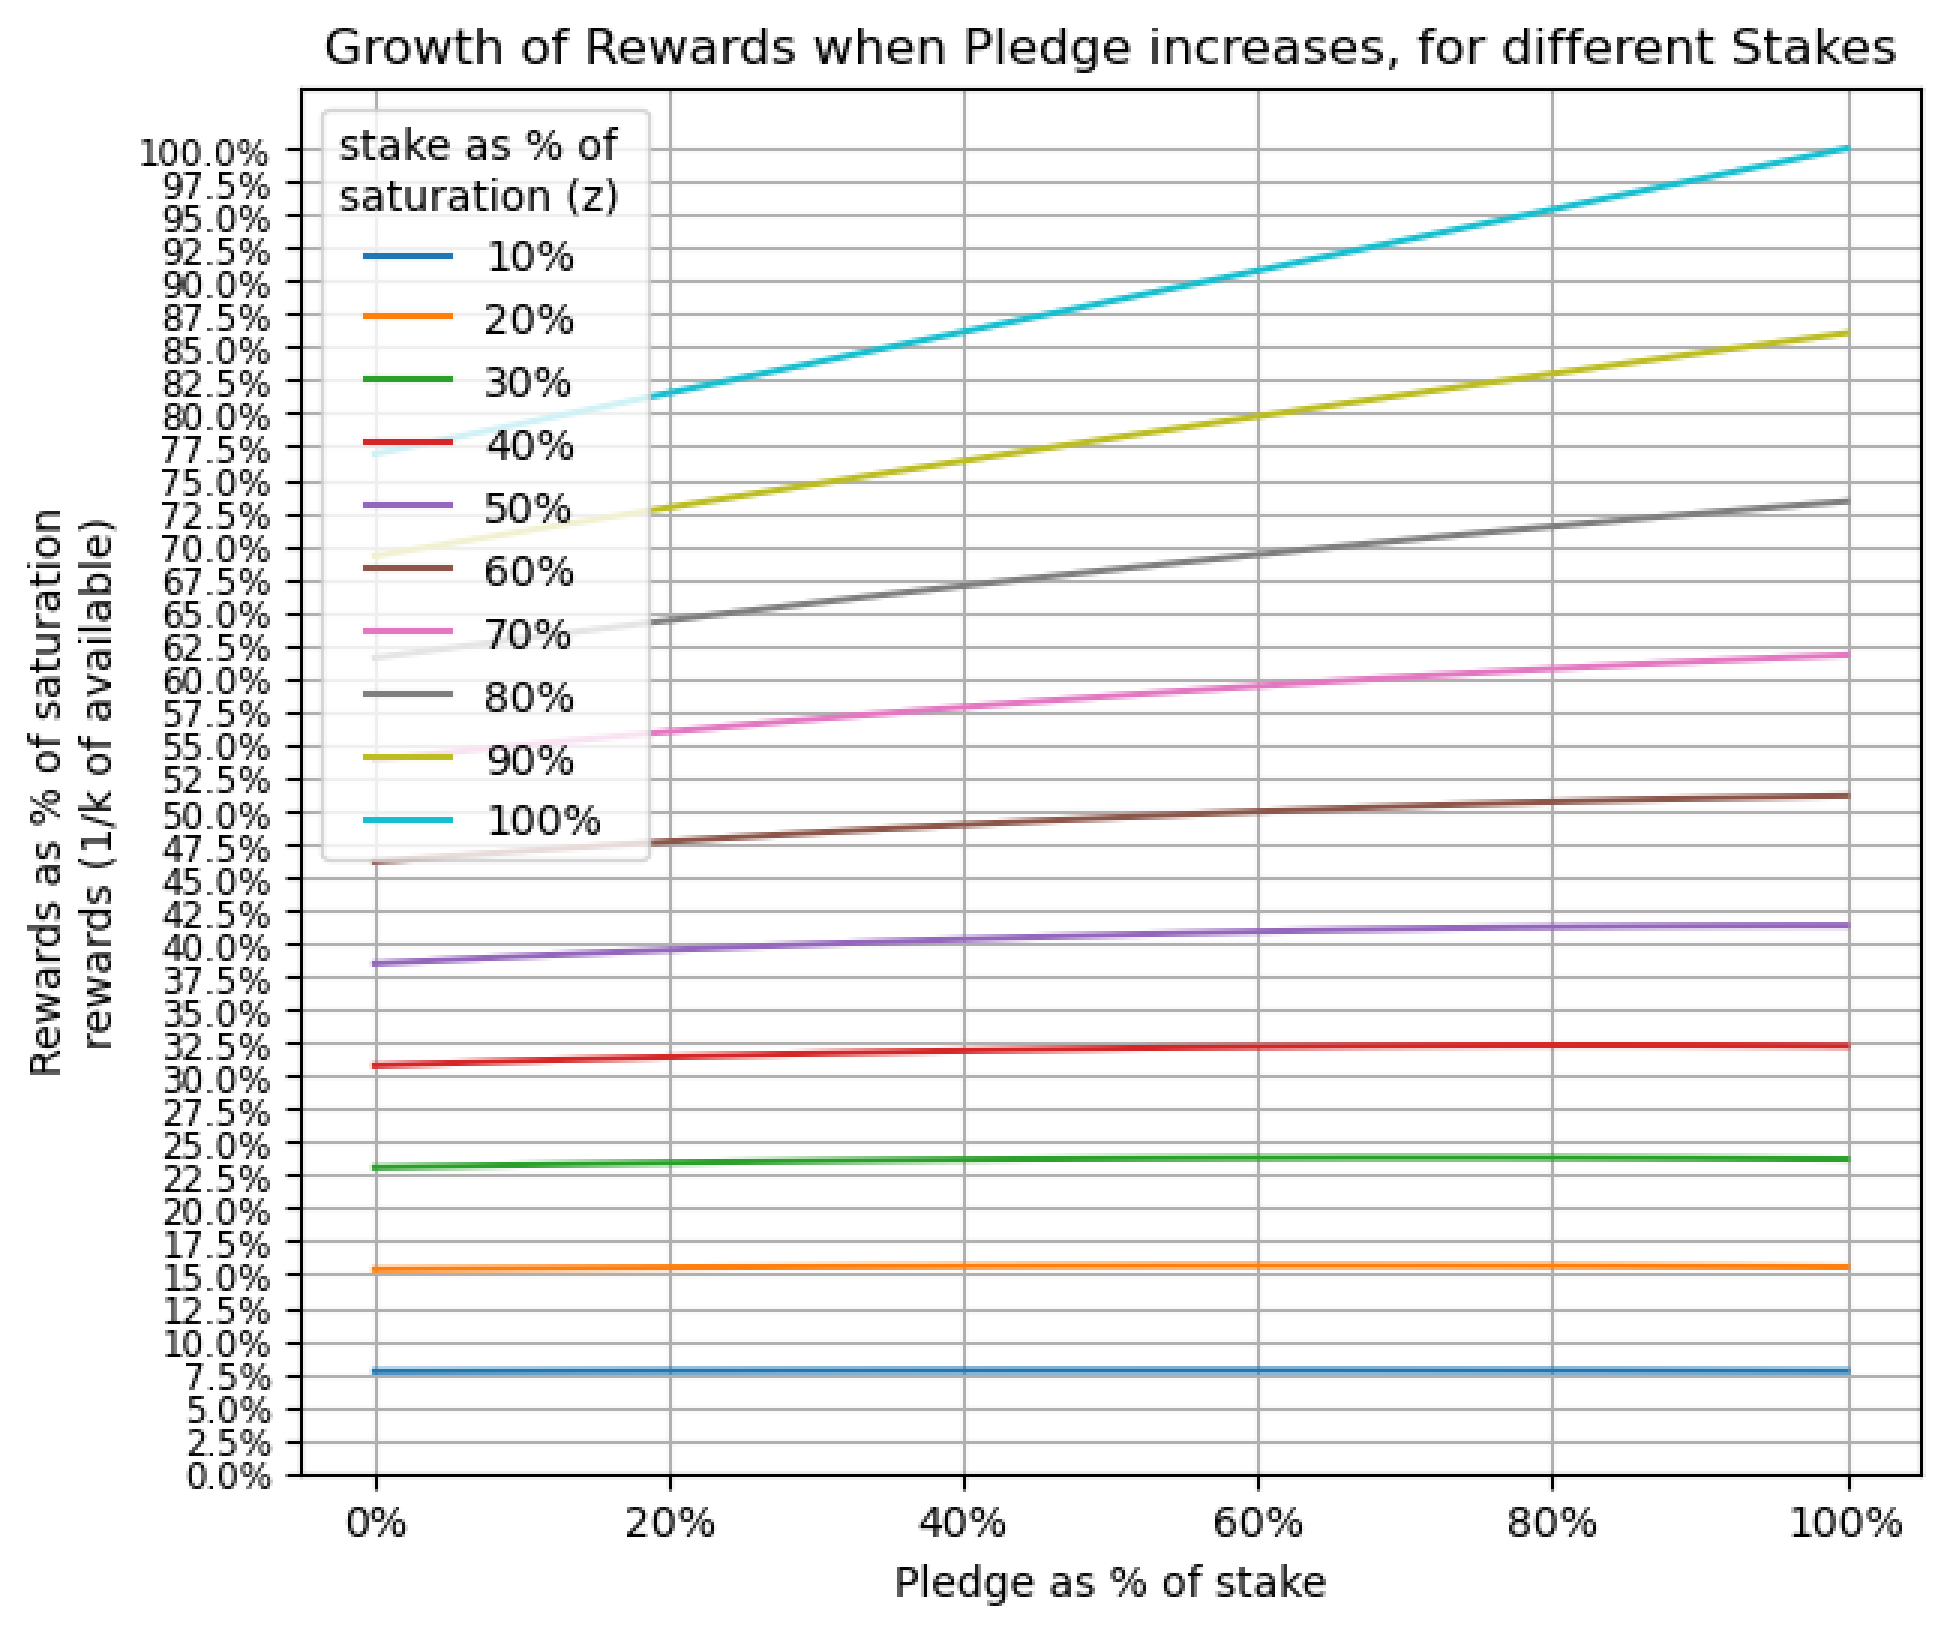
\includegraphics{figures/rewardswithstakepledgesimple}
\caption{\textbf{Rewards for different Stake and Pledge}. Stakes are represented
as fractions of saturation level ($S/k$), Rewards as fractions of
the maximum Reward ($1/k$ of the available rewards), Pledge as a
fraction of the Stake.}
\label{stakepledgesimple}
\end{figure}

\textbf{Description}. Pools with no pledge are penalized by considering
only a fraction $\frac{1}{1+a_{0}}$ of their share of the stake for
the purpose of reward computation. Since currently $a_{0}=0.3$, we
have $\frac{1}{1+a_{0}}\approx77\%$. To reduce this disadvantage,
it is not enough to increase the pledge. Pools need first to increase
their stake until it is a significant fraction of the saturation size,
to have an unambiguous increase of rewards from increasing the pledge.
For example, as one can see in Figure \ref{stakepledgesimple}, pools
with a stake which is $10\%$ of the saturated pool, \footnote{In the last few years the average saturation level has been around
70M ADA, so a 10\% pool had a stake of around 7M ADA. See also Section
\ref{subsec:Pool-Distribution}.} or less, receive around $7.7\%$ of the available rewards, rather
than a full $10\%$, even if they increase the pledge to 100\% of
the stake. A high pledge percentage can even marginally reduce rewards,
as explained later. For larger stakes, the benefit of a higher pledge
increases gradually, until the stake reaches $50\%$ of the saturation
level, when the pledge becomes beneficial in any amount. But only
fully saturated pools, by increasing the pledge towards 100\%, can
reach their full share of rewards ($1/k$).

\medskip{}

\textbf{Economic Rationale}. The current parameterization means that
large, individual pools built on own stake earn a higher return on
the pool's total stake, compared to small pools (no matter their pledge)
or to large pools based more on delegated stake. On one hand, this
can be undesirable in terms of inclusivity and decentralization. On
the other hand, this can be justified by the fact that small pools,
by having less skin in the game, are often less of a guarantee for
security. No matter their pledge, small pools remain an easy target
for an attacker, who can easily deploy resources higher than their
stake. It's more sensible for them to grow by attracting delegate
capital, in which case their contribution to security also grows,
thanks to the acquired capital, and to the need to attract delegators,
which also works as an incentive to honest behavior. Additionally,
large pools with small pledge can compensate a smaller total return
with the smaller size of the own capital they commit, leading to returns
on capital that can be much higher than the rewards of equivalent
fully pledged pools. The level of the two parameters $a_{0}$ and
$k$ has to be determined jointly to balance these different aspects. 

\subsection*{Some Maths}

The effect of $a_{0}$ and $k$ on the rewards of a pool depends on
the incentive formula
\begin{equation}
f\left(\alpha,z,\sigma,\lambda\right)=\frac{1}{1+\alpha}\left(\sigma+\alpha\lambda\frac{\sigma-\lambda\frac{z-\sigma}{z}}{z}\right),\label{eq:incentive formula}
\end{equation}
where we assume that pools are not saturated, but for simplicity do
not write this constraint explicitly. In this formula, $\alpha=a_{0}$
and $\sigma$ and $\lambda$ are the active stake and the own stake
or pledge of the pool. The quantities $\sigma$ and $\lambda$ are
both expressed as fractions of the circulating supply $S$ (aka total
stake), and so is the saturation level $z=\frac{S}{k}$. For example,
for a pool $x$ with a stake of $stake^{x}$ ADA, we have $\sigma=\frac{stake^{x}}{S}$.
The output of the formula is meant to represent the fraction of the
total available rewards that the pool will receive, save for a minor
adjustment that we will see later.

The formula is easier to interpret if rewrite it showing how the variables
defining the composition of the pool, $\sigma$ and $\lambda$, appear
in this function at different orders (or powers)
\begin{equation}
f\left(\alpha,z,\sigma,\lambda\right)=\frac{1}{1+\alpha}\sigma+\frac{\alpha}{1+\alpha}\left[\sigma\frac{\lambda}{z}+\sigma\left(\frac{\lambda}{z}\right)^{2}-z\left(\frac{\lambda}{z}\right)^{2}\right].\label{eq:firstfadjustment}
\end{equation}
We can also use more intuitive variables. Let us redefine the pledge
as a fraction of the stake of the pool, $\lambda_{\%}=\frac{\lambda}{\sigma}$,
and the stake of the pool as a fraction of the stake at saturation,
$\sigma_{\%}=\frac{\sigma}{z}$. 

\medskip{}

\textbf{Numerical Example} With these new variables, if the stake
at saturation is $70M$ and the stake of our pool is $7M$, with an
amount of pledge of $1.4M$, then $\sigma_{\%}=10\%$ and $\lambda_{\%}=20\%$.
The example is realistic. From maturity of the staking system around
epoch 300, until epoch 470, the average stake ranged between 6,893,338
and 7,950,258 ADA. In the same period, the average pledge ranged between
1,186,745 and 1,657,484 ADA. The circulating supply moved from almost
34B ADA to almost 37B. With $k=500$, the size of a saturated pool
averaged around 70M, so the above percentages represent a realistic
average Cardano pool. In the following we will use $\sigma_{\%}=10\%$
and $\lambda_{\%}=20\%$ as an example to fix ideas, and then we will
consider what happens for smaller or larger pools. 

With the new variables, 
\begin{align*}
f\left(\alpha,z,\sigma_{\%},\lambda_{\%}\right) & =\frac{1}{1+\alpha}\sigma_{\%}z+\frac{\alpha}{1+\alpha}\left[\sigma_{\%}^{2}\lambda_{\%}z-\sigma_{\%}^{2}\lambda_{\%}^{2}z+\sigma_{\%}^{3}\lambda_{\%}^{2}z\right]\\
 & =\left(\frac{1}{1+\alpha}\sigma_{\%}+\frac{\alpha}{1+\alpha}\left[\sigma_{\%}^{2}\lambda_{\%}-\sigma_{\%}^{2}\lambda_{\%}^{2}+\sigma_{\%}^{3}\lambda_{\%}^{2}\right]\right)z
\end{align*}
The last passage allows us to focus on the rewards of a pool as a
fraction of the rewards of the desired or optimal pool, which is fully
pledged and saturated, and therefore has size $z=1/k$, and also receives
$z=1/k$ of the total available rewards. Thus we define
\[
f_{\%}\left(\alpha,z,\sigma_{\%},\lambda_{\%}\right)=\frac{f\left(\alpha,z,\sigma_{\%},\lambda_{\%}\right)}{z}=\left(\frac{1}{1+\alpha}\sigma_{\%}+\frac{\alpha}{1+\alpha}\left[\sigma_{\%}^{2}\lambda_{\%}-\sigma_{\%}^{2}\lambda_{\%}^{2}+\sigma_{\%}^{3}\lambda_{\%}^{2}\right]\right).
\]
This makes it easier to understand how rewards depend on parameters.
The lead term in $f_{\%}$ is $\frac{1}{1+\alpha}\sigma_{\%}.$ If
there is no pledge, that's all a pool receives. For a pool with $\sigma_{\%}=10\%$,
this means that potential rewards are reduced by a factor $\frac{1}{1+\alpha}\approx0.77$,
for a total of $0.1*0.77=0.077=7.7\%$ of the rewards of the optimal
pool. 

Having a higher pledge fraction would not help so much at this size
of the pool, since all following terms are of larger order in $\sigma_{\%}$
and $\lambda_{\%}$ overall. When small fractions are multiplied or
raised to powers, their values decrease further. For the above example
pool, the second biggest term, of order 3 overall, is $\frac{\alpha}{1+\alpha}\sigma_{\%}^{2}\lambda_{\%}$
. With current $\alpha=0.3$, we get
\[
\frac{\alpha}{1+\alpha}\sigma_{\%}^{2}\lambda_{\%}=0.23*0.1^{2}*0.2=0.00046=0.046\%.
\]
This term is already very small compared to the leading term. The
next term is smaller and negative:
\[
-\frac{\alpha}{1+\alpha}\sigma_{\%}^{2}\lambda_{\%}^{2}=-0.23*10\%*10\%*20\%*20\%=-0.009\%
\]
The last term is of even higher order and even smaller in absolute
value, albeit positive:
\[
\frac{\alpha}{1+\alpha}\sigma_{\%}^{3}\lambda_{\%}^{2}=0.23*0.1^{3}*0.2^{2}=0.0009\%.
\]
Thus the contribution of the $20\%$ of own stake is to move rewards
from $7.7\%$ of the rewards of a saturated pool to $7.73\%$, a $0.03\%$
addition. If either the stake or the pledge were even smaller than
this average, the effect of the pledge would be even less relevant,
since all non-leading terms would be nearer to zero, the only term
where the order of the pledge is not smaller than the order of the
stake is the negative one.\footnote{As shown at the end of this section, this term can even result in
an increase in the pledge having a negative impact on the rewards.}

\medskip{}

\textbf{Large pools}. For larger pools the pledge becomes more relevant.
However, it is not until the stake $\sigma_{\%}$ approaches $50\%$
of the stake of the saturated pool that increasing the pledge has
a significant effect, with the stakes near to saturation having the
clearest benefit. It's easy to test that when $\sigma_{\%}=100\%$
of the saturation level, the formula becomes
\[
f_{\%}\left(\alpha,z,\sigma,\lambda\right)=\left(\frac{1}{1+\alpha}+\frac{\alpha}{1+\alpha}\lambda_{\%}\right)
\]
and increasing the pledge till $100\%$ of the stake increases the
rewards percentage linearly to $100\%$.

\medskip{}

\textbf{Conclusions}. Based on this analysis, the effect of a change
in $a_{0}=\alpha$ or $k=1/z$ is clearer. Reducing/increasing $a_{0}$
reduces/increases the penalization for pools that are smaller than
the size of the saturated pool, and makes the effect of increasing
the pledge less/more relevant, particularly for pools nearer to saturation
stake. Reducing/increasing $k$ increases/reduces the size of the
saturation stake, therefore changing the reference size that affects
the behavior of $a_{0}$. Furthermore, the saturation stake is also
the maximum size above which rewards are terminated. 

\begin{figure}[!ht]
\label{rewforstakepledge}\medskip{}

\begin{tabular}{cc}
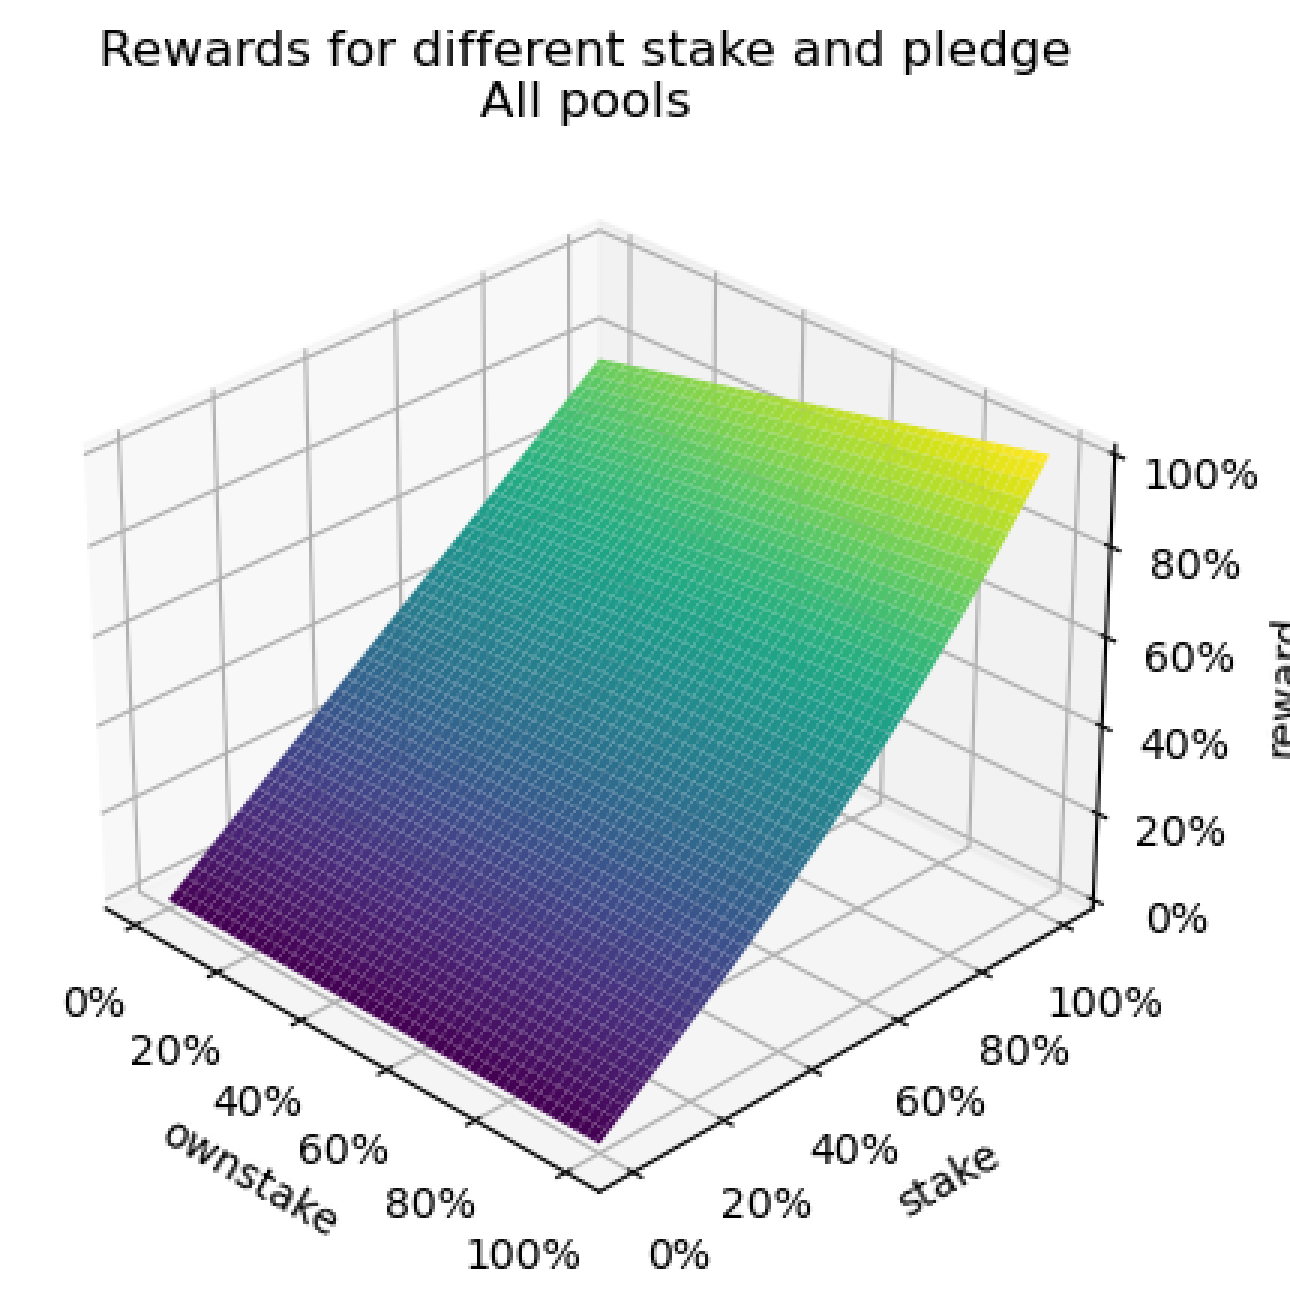
\includegraphics[scale=0.65]{figures/stakepledge_all} & 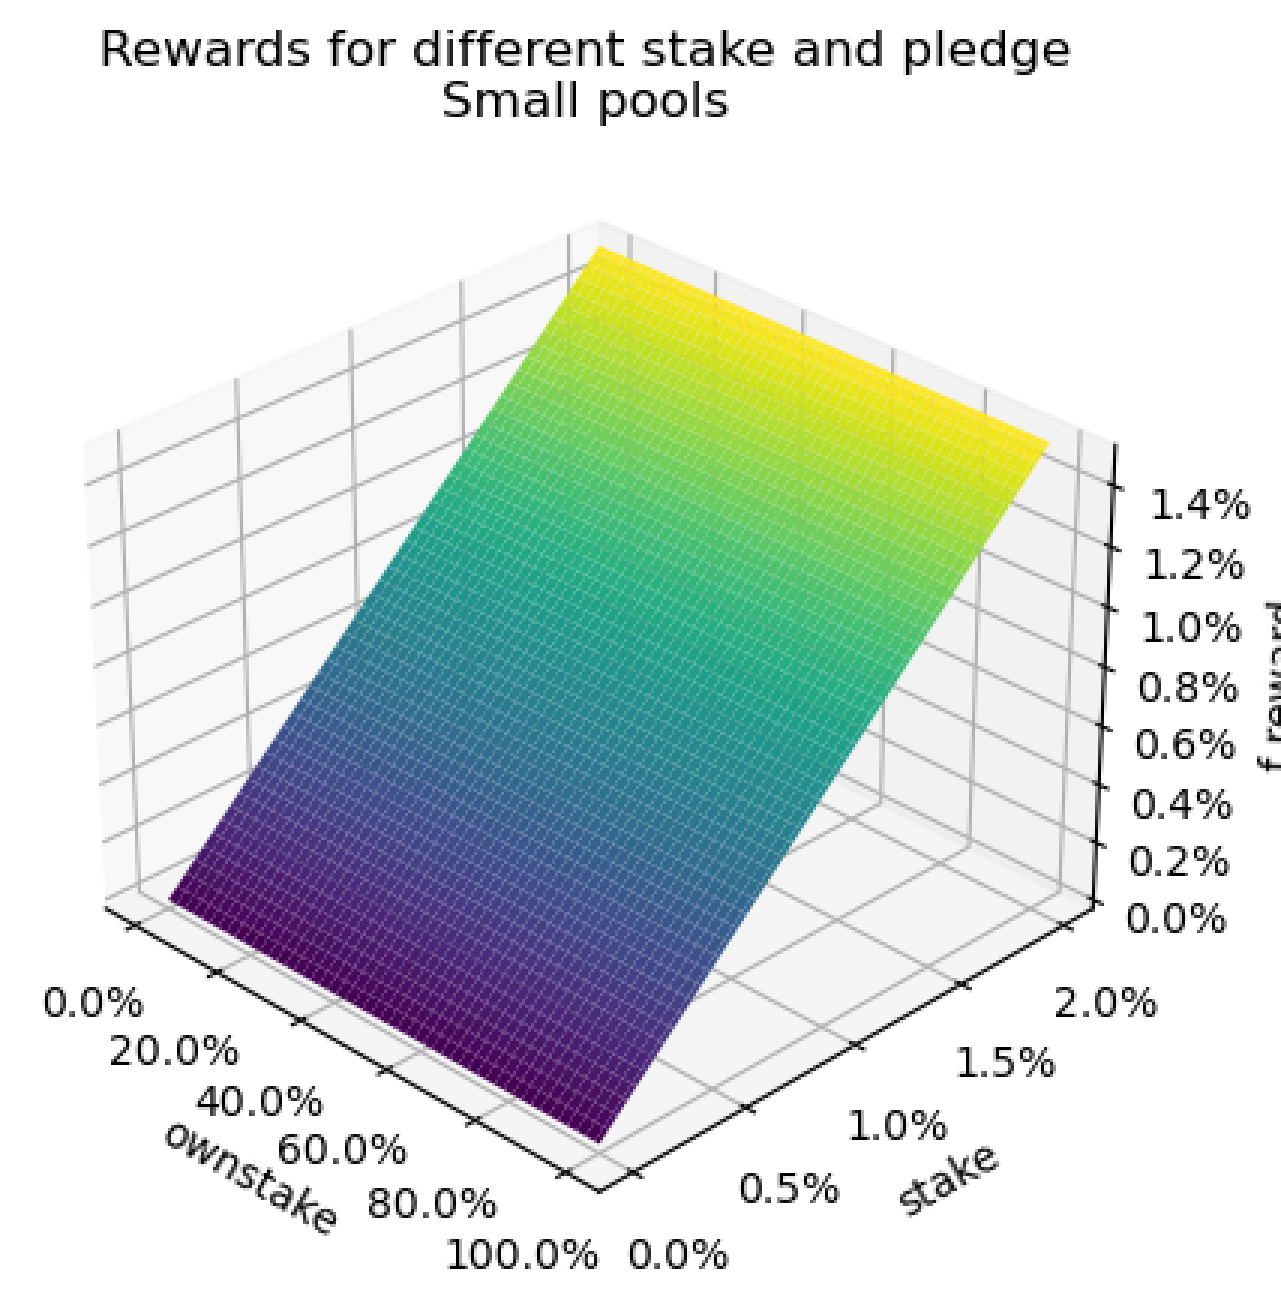
\includegraphics[scale=0.65]{figures/stakepledge_small}\tabularnewline
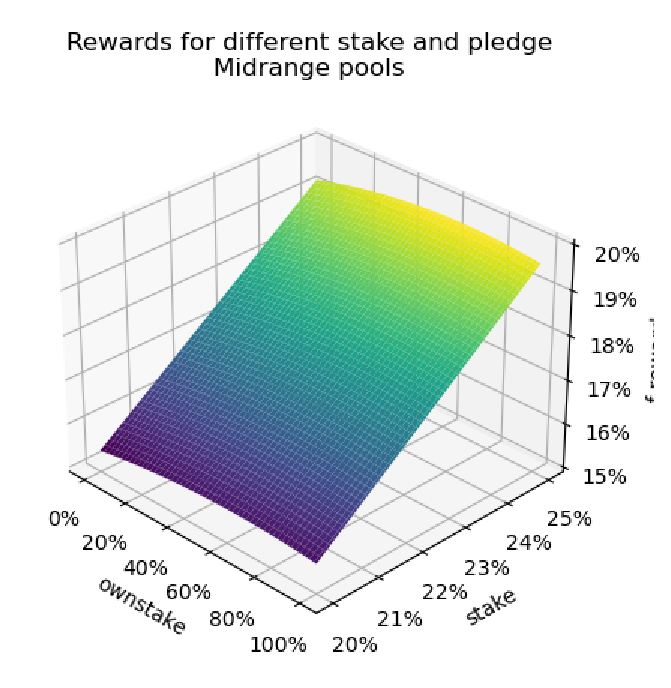
\includegraphics[scale=0.65]{figures/stakepledge_mid} & 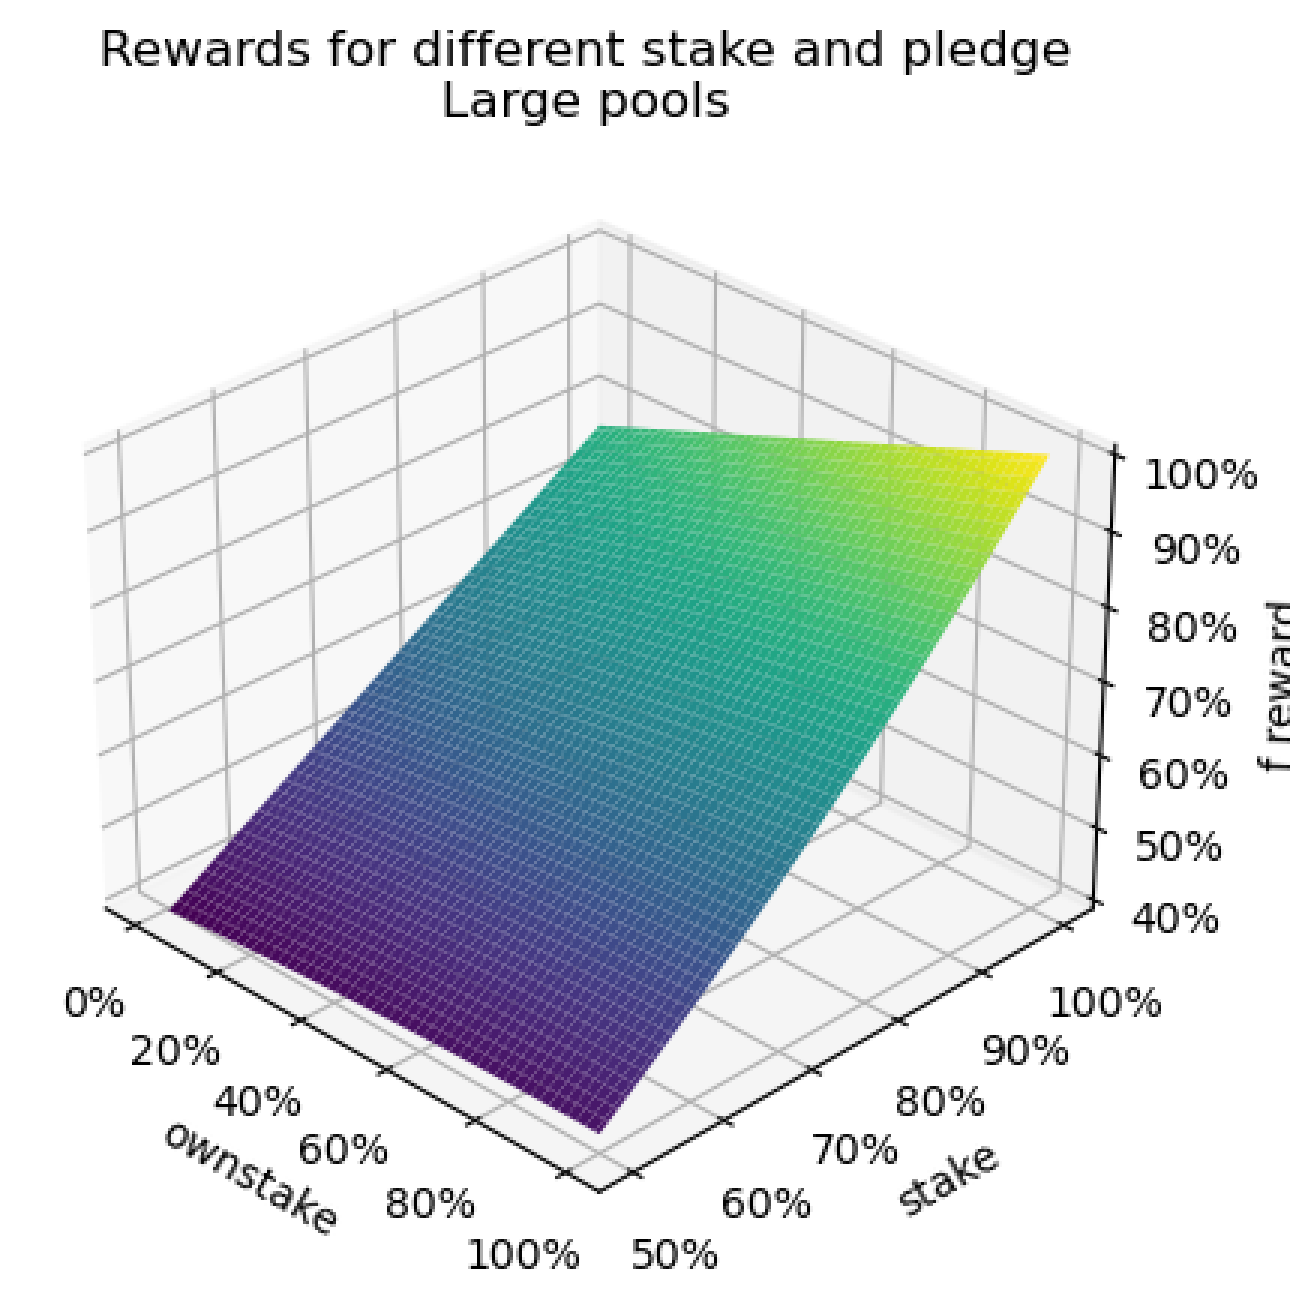
\includegraphics[scale=0.65]{figures/stakepledge_large}\tabularnewline
\end{tabular}\caption{\textbf{Rewards with stake and pledge, 3D.} Again, Rewards are percentages
of the reward of a fully pledged saturated pool, Stake are percentages
of the stake of the saturated pool, while Pledge is the percentage
of own stake in the stake.}
\end{figure}

The charts in \vref{rewforstakepledge} confirms. The top left chart
considers all possible levels of stake and pledge. For ease of analysis,
the other charts zoom in more narrow stake ranges, specifically pools
with stake from 0 to 2\% of the saturation stake (top right), stake
between 20\% and 25\% (bottom left), and finally stake from 50\% to
100\% (bottom right). We can also see that rewards decrease when pledge
increases, for fixed levels of the stake lower than 50\% of saturation.
This effect is explained in the following. 

\subsubsection*{Further Analysis}

It is useful to compute the first derivative of the rewards function
\eqref{eq:firstfadjustment} with respect to pledge $\lambda_{\%}$,
given by
\[
\frac{\partial f_{\%}\left(\alpha,z,\sigma_{\%},\lambda_{\%}\right)}{\partial\lambda_{\%}}=\left(\frac{\alpha}{1+\alpha}\left[\sigma_{\%}^{2}-2\sigma_{\%}^{2}\lambda_{\%}+2\sigma_{\%}^{3}\lambda_{\%}\right]\right).
\]
A function grows when its first derivative is positive, and goes down
if the derivative turns negative. The first derivative turns from
positive to negative when
\[
\lambda_{\%}\geq\frac{1}{2\left(1-\sigma_{\%}\right)}\equiv\lambda_{\%}^{*}\left(\sigma_{\%}\right)
\]
This means that rewards grow with $\lambda_{\%}$ until $\lambda_{\%}=\lambda_{\%}^{*}$,
but, for pledges larger than this value, increasing the pledge reduces
rewards. The value $\lambda_{\%}^{*}\left(\sigma_{\%}\right)$ at
which a higher pledge proportion starts reducing rewards depends on
$\sigma_{\%}$, the size of the pool relative to the saturated pool.
$\lambda_{\%}^{*}\left(\sigma_{\%}\right)$ grows with $\sigma_{\%}$,
and when $\sigma_{\%}$=50\% we have $\lambda_{\%}^{*}$=100\%. Only
at this level of stake increasing the pledge always increases rewards,
since in practice pledge cannot be higher than 100\% of the stake.
For lower stakes, there will always be a level of the pledge that
it is better not to reach, since beyond that level more pledge means
less rewards, as shown in \vref{deriv}. For $\sigma_{\%}$=1\% the
absolute effect of the pledge is so small that it's hardly relevant
if the effect is positive or negative. But for $\sigma_{\%}$=10\%
and then $\sigma_{\%}$=20\% it becomes increasingly visible that,
when pledge is increased, rewards grow slightly until the point when
the derivative crosses the x-axis and becomes negative. Beyond that
point, rewards decrease slightly if the pledge is increased. For $\sigma_{\%}\geq$50\%,
the rewards become uniformly increasing with pledge. Indeed, at $\sigma_{\%}=$50\%
the first derivative crosses the x-axis and becomes negative only
at at 1, that is 100\% pledge. 

\begin{figure}[!ht]
\label{deriv}%
\begin{tabular}{cc}
\includegraphics[width=7cm,height=5cm]{figures/pledgederivative_sig0\lyxdot 01} & \includegraphics[width=7cm,height=5cm]{figures/pledgederivative_sig0\lyxdot 1}\tabularnewline
\includegraphics[width=7cm,height=5cm]{figures/pledgederivative_sig0\lyxdot 2} & \includegraphics[width=7cm,height=5cm]{figures/pledgederivative_sig0\lyxdot 5}\tabularnewline
\end{tabular}\caption{\textbf{Behavior of Rewards with pledge and its 1st derivative. }Showing
different cases for different $\sigma_{\%},$ i.e. different stakes
expressed as fixed percentages of saturation, showing in each chart
both the function and its derivative with respect to the proportion
$\lambda_{\%}$ of pledge.}
\end{figure}


\section{The effect of Stake definitions}

The incentives emerging from the application of \eqref{eq:incentive formula}
to all pools are not the last adjustment made to available resources
before paying them out as rewards. As \citet{webdocgeneral} says,
``the rewards that are produced by this formula are now adjusted
by pool's performance: we multiply by $\frac{\beta}{\sigma_{a}}$,
where $\beta$ is the fraction of all blocks produced by the pool
during the epoch and $\sigma_{a}$ is the stake delegated to the pool
relative to the active stake ''. The more technical reference \citet{Kant2020Delegation}
says ``The actual rewards take the apparent performance into account,
and are given by $\bar{p}*f\left(\right)$. Since $\bar{p}=\beta/\sigma$,
this nearly amounts to replacing $\sigma$ by $\beta$ in $f\left(\right)$,
i.e. to rewarding pools based on the number of blocks that they produced''.

Let us define this final adjustment precisely. It consists of multiplying
the output of the incentive formula for a pool $x$, with a stake
of $stake^{x}$ ADA, by 
\begin{equation}
\frac{N^{x}}{N}\frac{active}{stake^{x}}\label{eq:second adjustment}
\end{equation}
where $N^{x}$ the number of blocks produced by the pool $x$, $N$
is the total number of blocks given by the sum of $N^{x}$ for all
pools, and $active$ is the total amount of stake doing validation,
given by the sum of $stake^{x}$ for all pools. Individually, this
adjustment takes into account of the technological efficiency of a
pool in producing blocks. In terms of aggregate effect on the total
amount of rewards distributed, the adjustment is small. According
to the consensus protocol, in an idealized setting where all pools
operate with perfect efficiency and the realization of randomness
matches probabilistic expectations, the pool's fraction of blocks
$\frac{N^{x}}{N}$ would track the pool's fraction of stake $\frac{stake^{x}}{active}$
and \eqref{eq:second adjustment} would be very near to 1. In practice,
this remains true on average.

Yet, introducing explicitly the pool performance and the active stake
in the adjustments helps us understand them better. We saw in Section
1 that the incentive formula \eqref{eq:incentive formula} depends
on the relative stake defined as a fraction $\sigma=\frac{stake^{x}}{S}$
of the total stake or circulating supply $S$. This definition of
the weight of a pool used for rewards is different from the one used
in the protocol to select pools for validation, which is instead $\sigma_{a}=\frac{stake^{x}}{active}$,
determining $\frac{N^{x}}{N}.$ The latter are definitions of the
relative weight of a pool that sum up to 1 if one considers all pools.
Instead, $\sigma=\frac{stake^{x}}{S}$ weights do not sum up to 1
when one considers all pools, but just to
\[
p=\frac{active}{S}.
\]

If $\sigma_{a}$ was used instead of $\sigma$, there would be no
adjustment if all pools were fully saturated and pledged. Instead
with $\sigma$, even if all pools were ideal, there would be in any
case an adjustment to the total amount of resources before paying
them out as rewards, given by $p$. Thus in practice the adjustments
include not only the incentives for the pools to have the desired
size, pledge and efficiency, but also a rescaling by $p$. 

It useful to represent the aggregate effect of the adjustments, given
by summing $\frac{N^{x}}{N}\frac{active}{stake^{x}}f\left(\alpha,z,\sigma^{x},\lambda^{x}\right)$
for all pools, as $p*f$, where $p$ is always the ratio between active
stake and circulating supply, while $f$ is derived implicitly from
knowledge of the aggregate adjustment and of $p$. Since these quantities
can change at every epoch $i$, we add an epoch index and write

\[
Rewards_{i}=f_{i}*p_{i}*AvailableRewards_{i}.
\]
At the end of this Section we will see that this is almost equivalent
to compute $f_{i}$ by replacing, for each epoch and each pool, $\sigma_{i}^{x}=\frac{stake_{i}^{x}}{S_{i}}$
with $\frac{stake_{i}^{x}}{active_{i}}$ in the incentive formula,
then sum up these adjustments $f\left(\alpha,z,\frac{stake_{i}^{x}}{active_{i}},\lambda_{i}^{x}\right)$
for all pools. Having redefined the stake, now this aggregate adjustment
can reach 1 if pools have the desired size and are fully pledged,
therefore it is finally rescaled by $p.$

\textbf{Economic relevance}. Why the final passage? What's the effect
of rescaling by $p$? This final rescaling changes the behavior of
Rewards when the active stake moves. Without rescaling, the total
amount of rewards paid out in every epoch would be adjusted only by
$f$ and would not change when the active stake changes. If the active
stake went down, the remaining stake would share the same total rewards
with a higher yield for each unit of stake, and the other way around
if the stake increased. 

Rescaling by $p$ neutralizes this effect, by reducing rewards proportionally
when the active stake decreases, and increasing them proportionally
when the active stake goes up. The advantages of this rescaling are
the stability of rewards for each pool, and more importantly the elimination
of any incentive for validators to reduce the active stake in order
to increase their yield, for example by delaying the approval of new
pools. 

From a tokenomic point of view, there are other considerations to
make. In many other popular blockchains such as Bitcoin, the amount
of rewards is set in advance and the participation rate (e.g. hashing
power in proof-of-work) does not impact the total amount distributed.
In Cardano Rewards could work like in Bitcoin. The amounts released
in every period are parameterized in both chains. Also in Cardano,
the available reward could be all distributed after the incentive
formula has been applied, without adjusting them by the level of stake,
i.e. without adjusting them by $p$. 

This could stabilize the participation of validators. If the active
stake went down, the Reward yield for unit of stake would increase,
attracting more validators. This could be useful in case of excessive
competition for the use of stake from the DeFi market or any other
successful application, not to mention stronger competition from external
activities, such as validation in other chains or fiat interest rates.
In this case it would be important to check that $p$, by reducing
total rewards when stake decreases, does not lead a so-called ``pro-cyclical
effect'', which means contributing to a further stake decrease. This
needs monitoring and analysis through time, under the constraint that
any possible improvement must remain free from manipulation and aware
of the max cap.

\textbf{Historical behavior.} In Figure \ref{fandp} we can see the
value taken by both $f_{i}$ and $p_{i}$ during the last few years.
We see that, as expected, both are lower than one. A bit more surprisingly,
we can notice that the $p$ fraction is always lower than the $f$
fraction, therefore $p$ reduces rewards more than the specific pool
incentives $f$ in every epoch. It is also the largest contributor
to the volatility of aggregate rewards over time, with even an upward
jump after epoch 325,\footnote{Jumps in staking are usually associated to large players, such as
exchanges, starting or terminating their participation in staking.} and a smoother but bigger decline after epoch 400.

\begin{figure}[!ht]
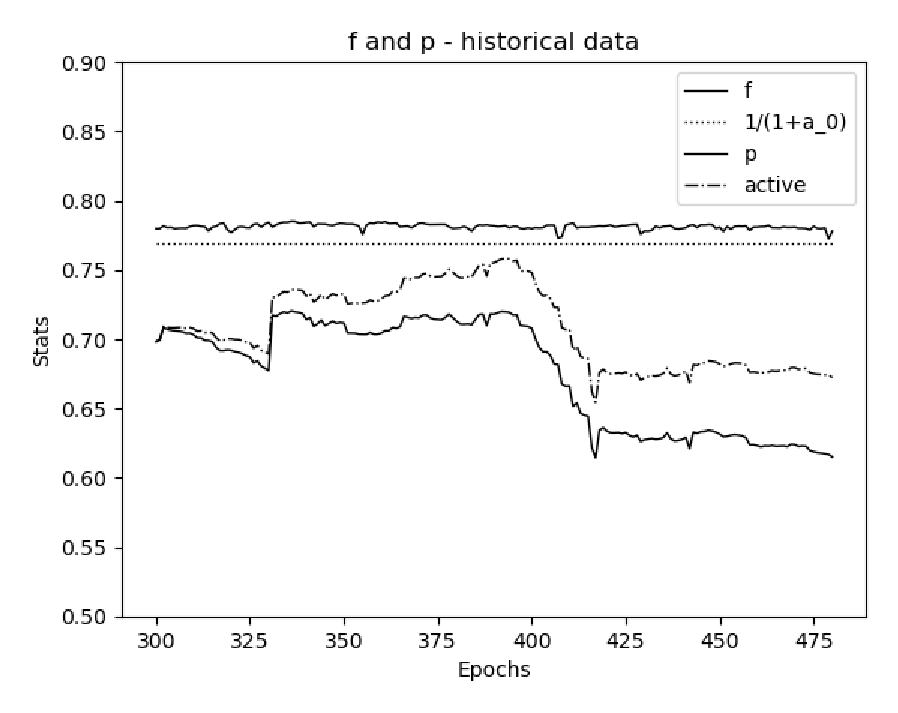
\includegraphics[scale=0.98]{./figures/f_and_p.eps}\caption{\textbf{Reward adjustment f and p in practice }The chart shows $p$
and $f$ as extracted from the actual level of rewards, beside the
leading term in $f$, $\frac{1}{1+a_{0}}\approx77\%$, and the active
stake component of $p$.}
\label{fandp}
\end{figure}

We can also distinguish the effects on $p$ of variations in active
stake from the effect of variations in circulating supply, by comparing
$p$ with $active$ in Figure \ref{fandp}. That is the active stake
not divided by the circulating supply in every epoch, but by the circulating
supply at epoch 300, the first epoch considered, to have the same
starting point as $p$. We see that the active stake is more stable
than $p$, which is the ratio between active stake and circulating
supply. Circulating supply increases in normal times. Using it as
the denominator, makes the $p$ ratio decrease more than active stake,
and contributes to its volatility. This confirms the need to analyze
and monitor the definitions of stake relevant to tokenomics.

Figure \ref{fandp} also raises the question of why $f$ is so close
to the $\frac{1}{1+\alpha}$ minimum. As we saw in Section 1, this
is the level of rewards that applies to pools with zero pledge. The
following mathematical description will help understand this, and
a further clarification will come from the analysis of the distribution
of stake and pledge across pools. 

\textbf{Some Maths}. Here we explain the approximate equivalence between
$f$ and the aggregate effect of incentives that we obtain if we replace
$\sigma^{x}=\frac{stake^{x}}{S}$ with $\sigma_{a}^{x}=\frac{stake^{x}}{active}$
in the incentive formula. We start from the formula as given in \eqref{eq:firstfadjustment}
and write it to show its components as 
\begin{align}
f\left(\alpha,z,\sigma^{x},\lambda^{x}\right) & =\sigma^{x}\frac{1}{1+\alpha}+\sigma^{x}\underset{}{\frac{\alpha}{1+\alpha}\left[\frac{\lambda^{x}}{z}+\left(\frac{\lambda^{x}}{z}\right)^{2}\right]}-\underset{}{\frac{\alpha}{1+\alpha}z\left(\frac{\lambda^{x}}{z}\right)^{2}}.\label{eq:rewards reformualted again}\\
 & =\frac{stake^{x}}{S}\frac{1}{1+\alpha}+\frac{stake^{x}}{S}\gamma\left(\alpha,z,\lambda^{x}\right)-\varepsilon\left(\alpha,z,\lambda^{x}\right).\nonumber 
\end{align}
Remembering the analysis in the first section, we see the stake relative
to total supply multiplied first by $\frac{1}{1+\alpha}$, and then
by a function $\gamma\left(\alpha,z,\lambda^{x}\right)$ which is
likely to be smaller, and finally we have a negative term $\varepsilon\left(\alpha,z,\lambda^{x}\right)$,
depending on the square of the relative pledge and only indirectly
on the stake. This term is usually very small, or simplifies with
part of $\gamma$, as we saw above. If we now add the second adjustment,
we obtain

\[
\frac{N^{x}}{N}\frac{active}{stake^{x}}\left[\frac{stake^{x}}{S}\frac{1}{1+\alpha}+\frac{stake^{x}}{S}\gamma\left(\alpha,z,\lambda^{x}\right)-\varepsilon\left(\alpha,z,\lambda^{x}\right)\right]
\]
Noticing that $stake^{x}$ cancels out, we get
\[
\frac{active}{S}\left[\frac{N^{x}}{N}\frac{1}{1+\alpha}+\frac{N^{x}}{N}\gamma\left(\alpha,z,\lambda^{x}\right)-\hat{\varepsilon}\left(\alpha,z,\lambda^{x}\right)\right],
\]
where $\hat{\varepsilon}$, which is $\varepsilon$ modified by the
final adjustment, is still expected to be small or to nearly cancel
out. Based on this, we can understand the approximation mentioned
by \citet{Kant2020Delegation} ``this nearly amounts to rewarding
pools based on the number of blocks that they produced''. Adding
the convergence of $\frac{N^{x}}{N}$ to $\frac{stake^{x}}{active}$
on average, we get the following approximation of the aggregate reward
adjustment
\begin{align*}
 & \sum_{x}\frac{active}{S}f\left(\alpha,z,\frac{stake^{x}}{active},\lambda^{x}\right)\\
= & \frac{active}{S}\sum_{x}\left[\frac{stake^{x}}{active}\frac{1}{1+\alpha}+\frac{stake^{x}}{active}\gamma\left(\alpha,z,\lambda^{x}\right)-\hat{\varepsilon}\left(\alpha,z,\lambda^{x}\right)\right]\\
= & \frac{active}{S}\left[\frac{1}{1+\alpha}+\sum_{x}\frac{stake^{x}}{active}\gamma\left(\alpha,z,\lambda^{x}\right)-\sum_{x}\hat{\varepsilon}\left(\alpha,z,\lambda^{x}\right)\right],
\end{align*}
where in square brackets we have the approximation of $f$, showing
its terms from the most relevant to the one expected to be the smallest. 

\section{Pool Distribution and Rewards\label{subsec:Pool-Distribution}}

The historical evidence in Figure \ref{fandp} provides a striking
confirmation of the goodness of the approximation just computed, and
of the expectation that $\frac{1}{1+\alpha}=\frac{1}{1+a_{0}}\approx77\%$
is the dominant component of the $f$ adjustment. The other components
of $f$, which should increase the rewards above the $\frac{1}{1+a_{0}}$
minimum, accounted for less than 2\% in the last few years. This evidence
that aggregate rewards were little higher than the amount that applies
to pools with no pledge needs to be rooted in the distribution of
the staking pools during the period. We analyze this in the following,
keeping the analysis simple and based on few basic statistics. 

\begin{figure}[!ht]
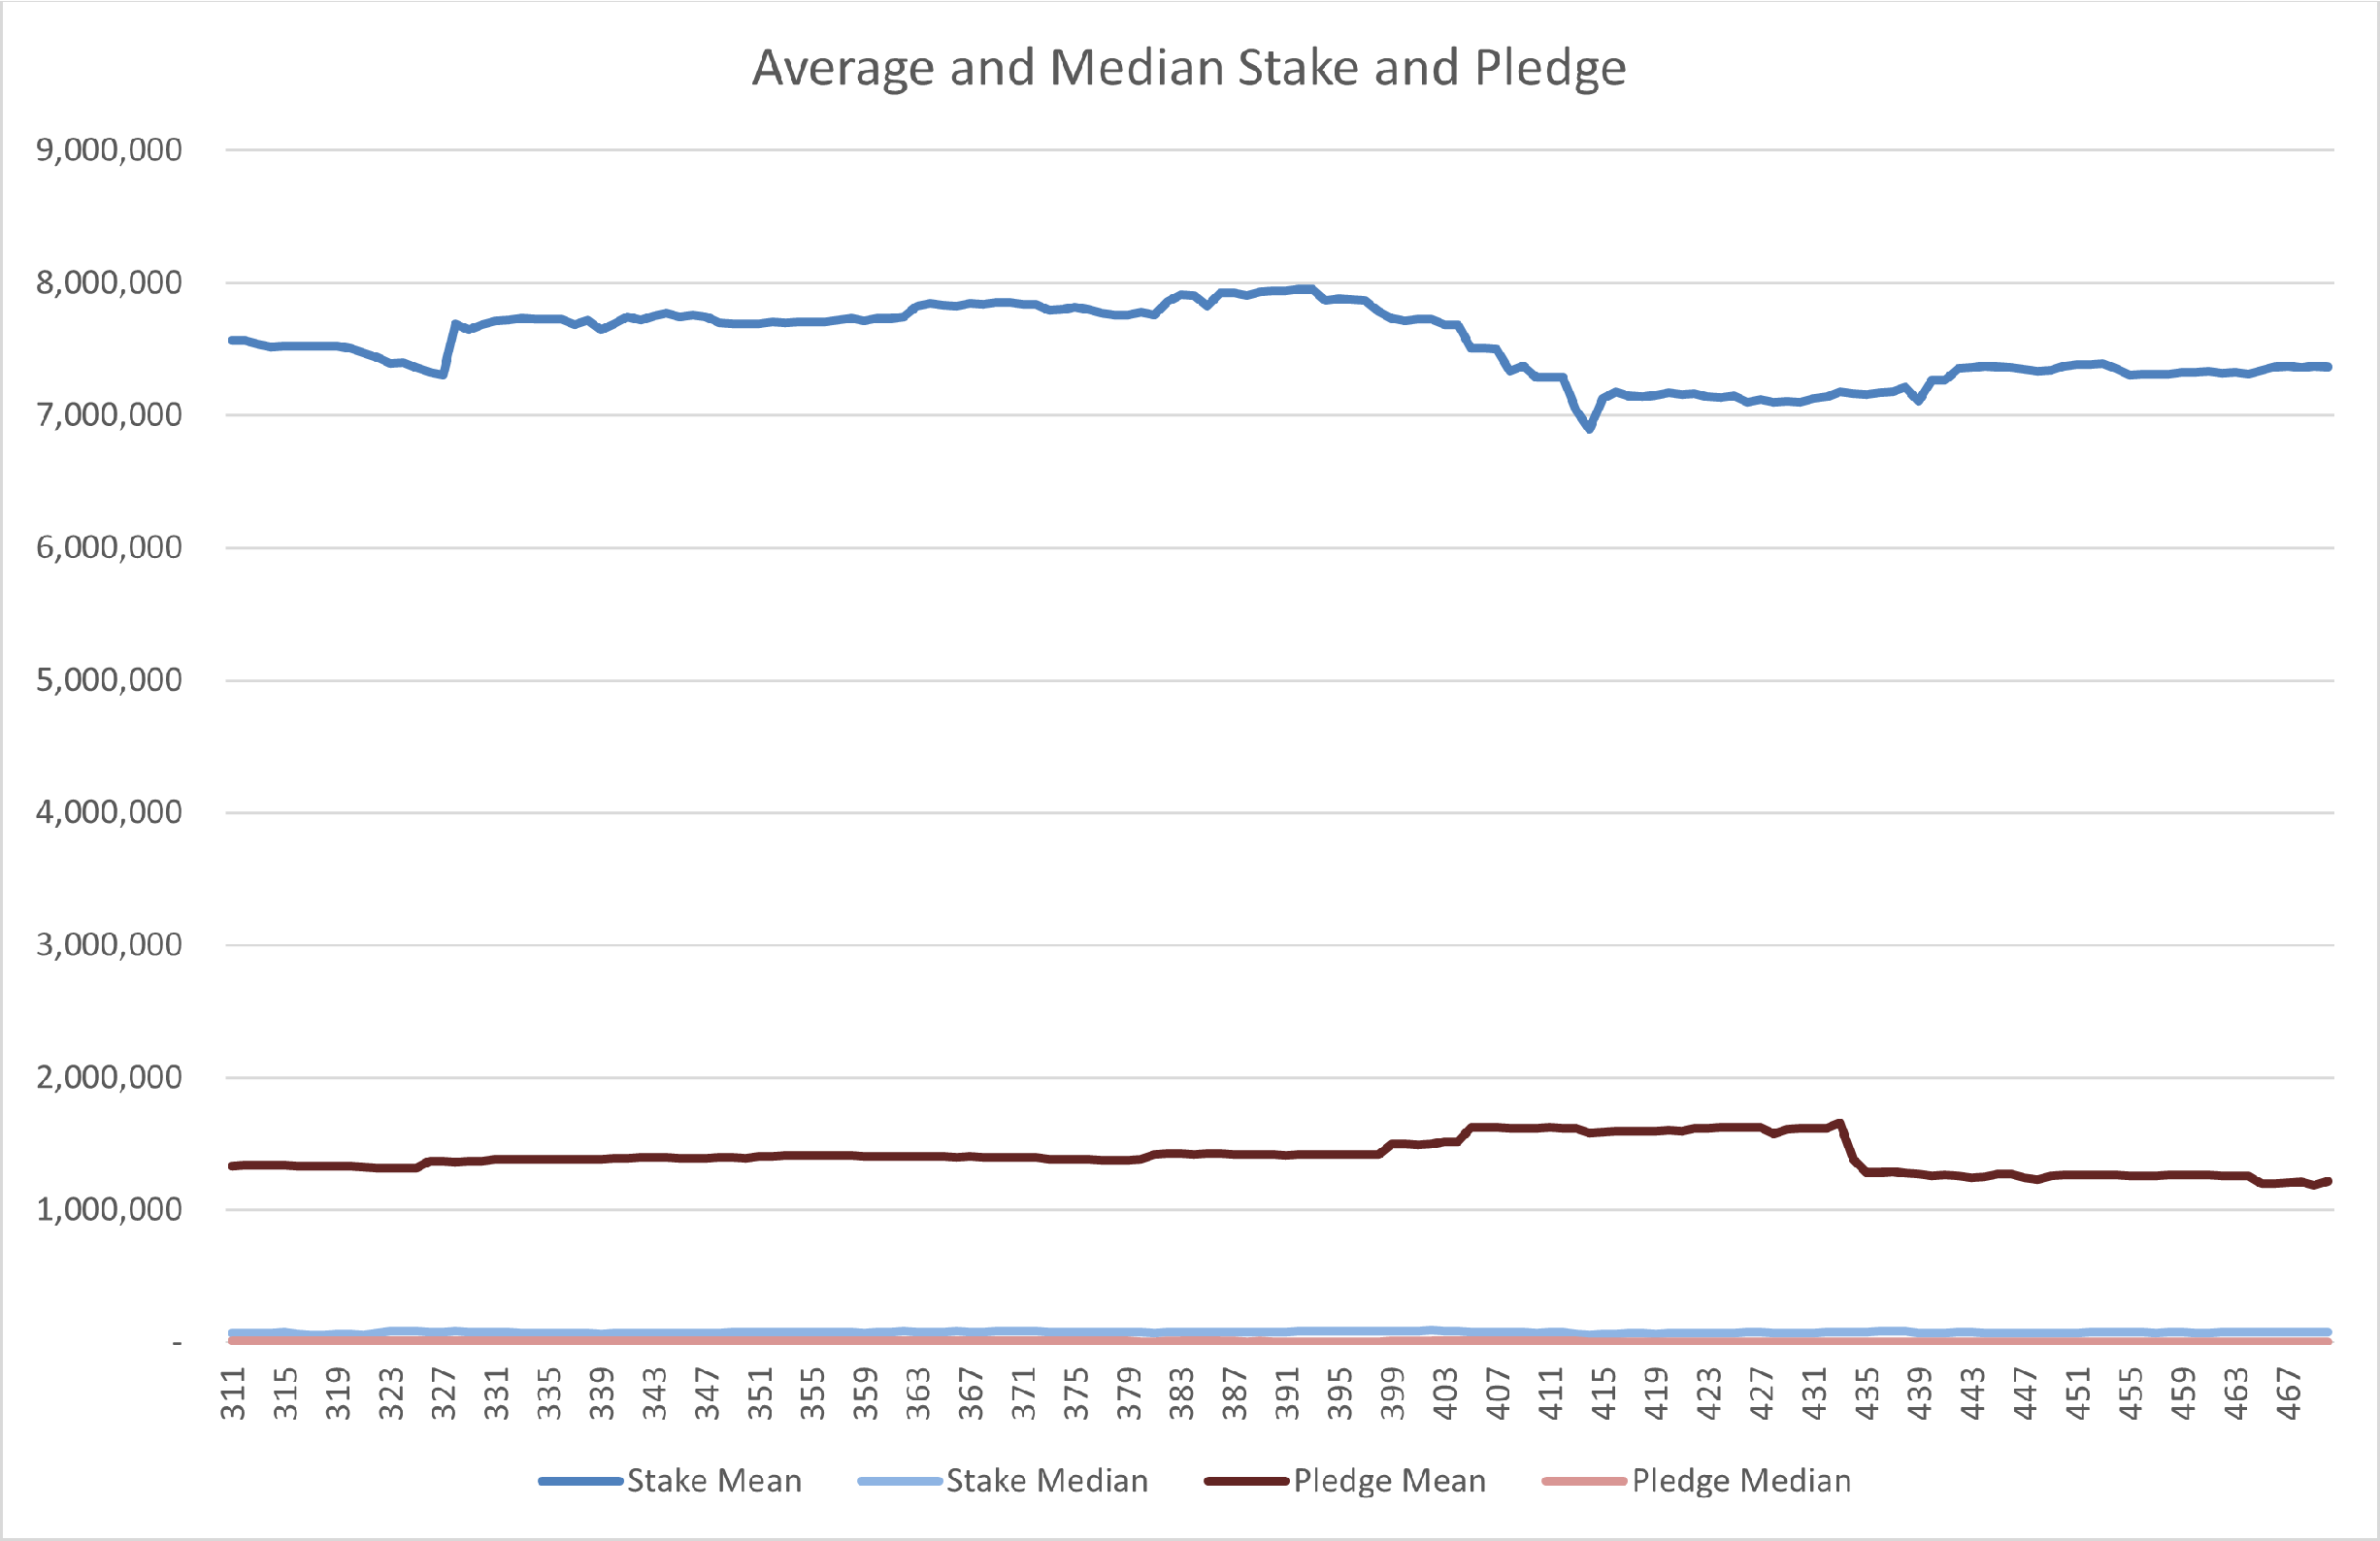
\includegraphics[scale=0.7]{figures/stakepledgemeanmedian}\caption{\textbf{Average and Median Stake and Pledge. }The figure covers the
period from epoch 311-470.}
\label{fig_average_median_pools}
\end{figure}

\textbf{Statistics}. We see in Figure \ref{fig_average_median_pools}
that the average pool had a stake between 7 and 8 Million ADA. The
average pledge was around 1.5 Million ADA. This amount of own tokens
is not very high, but it is significantly above zero. We know from
the initial analysis that the pledge has different effects on pools
with different stake, so we need to know more than the average stake
and pledge, to understand why there is so little effect from the pledge.
Since the median is the value with 50\% higher observations and 50\%
lowest observations, median values could add relevant information,
but here we see that median stake and pledge are very small, due to
the presence of very many very small pools. So median data do not
help understand the real distribution of the pools in terms of stake
and pledge size. 

Let's build slightly more granular, and more targeted, statistics.
In Figure \eqref{fig_pools_by_stake} the upper chart shows how the
stake has been distributed across different classes of stake,
\[
\left[0-7M\right],\left[7M-14M\right],\left[14M-21M\right]...\left[63M-70M\right],\left[70M-77M\right].
\]

They correspond approximately to 
\[
\left[0-10\%\right],\left[10\%-30\%\right],\left[20\%-30%\%
\right]...\left[90\%-100%\%
\right],\left[100\%-110%\%
\right]
\]
 of the average saturation level of the period, that ranges between
67M and 73M ADA. The class of pools with highest stake, $\left[70M-77M\right]$,
was above the saturation stake in the first years used in the analysis.
But the saturation stake increases with circulating supply, so the
number of pools in this class grows with the increase of the saturation
stake to 70M and above. Any higher stake has been added to this last
class, considering that no additional rewards are given to pools larger
than saturation. 
\begin{figure}[!ht]
\medskip{}

\begin{tabular}{c}
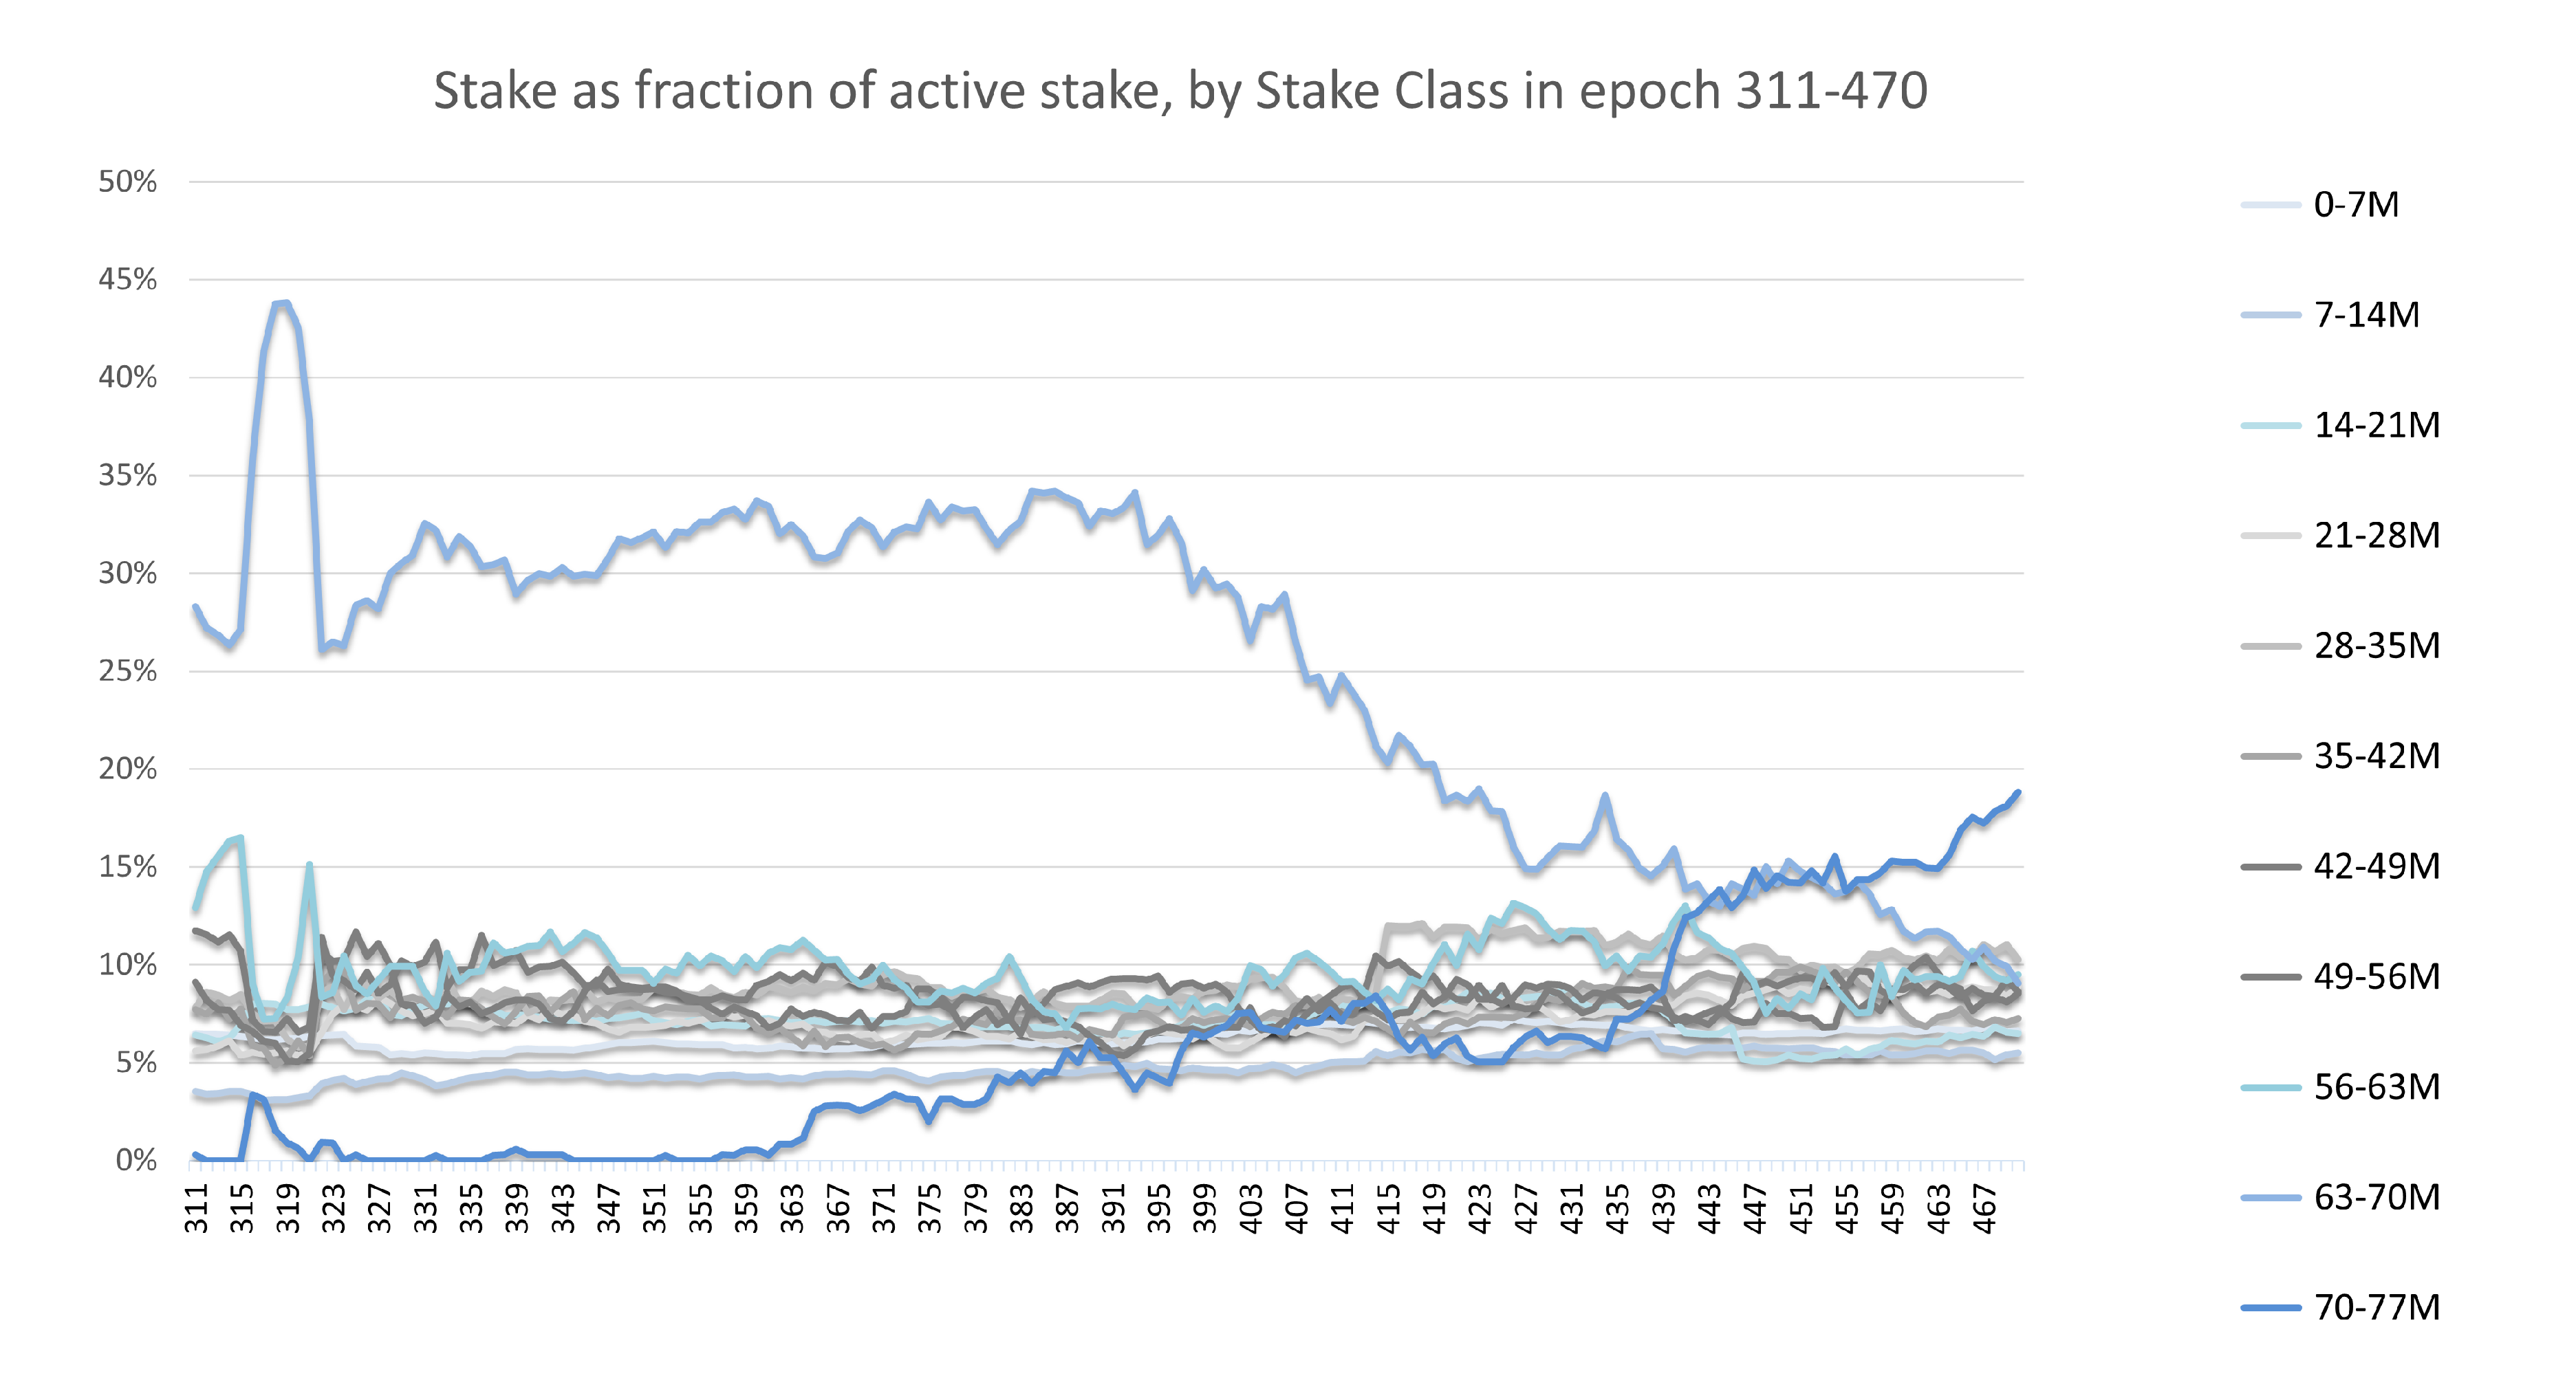
\includegraphics[scale=0.44]{figures/stakebyrange}\tabularnewline
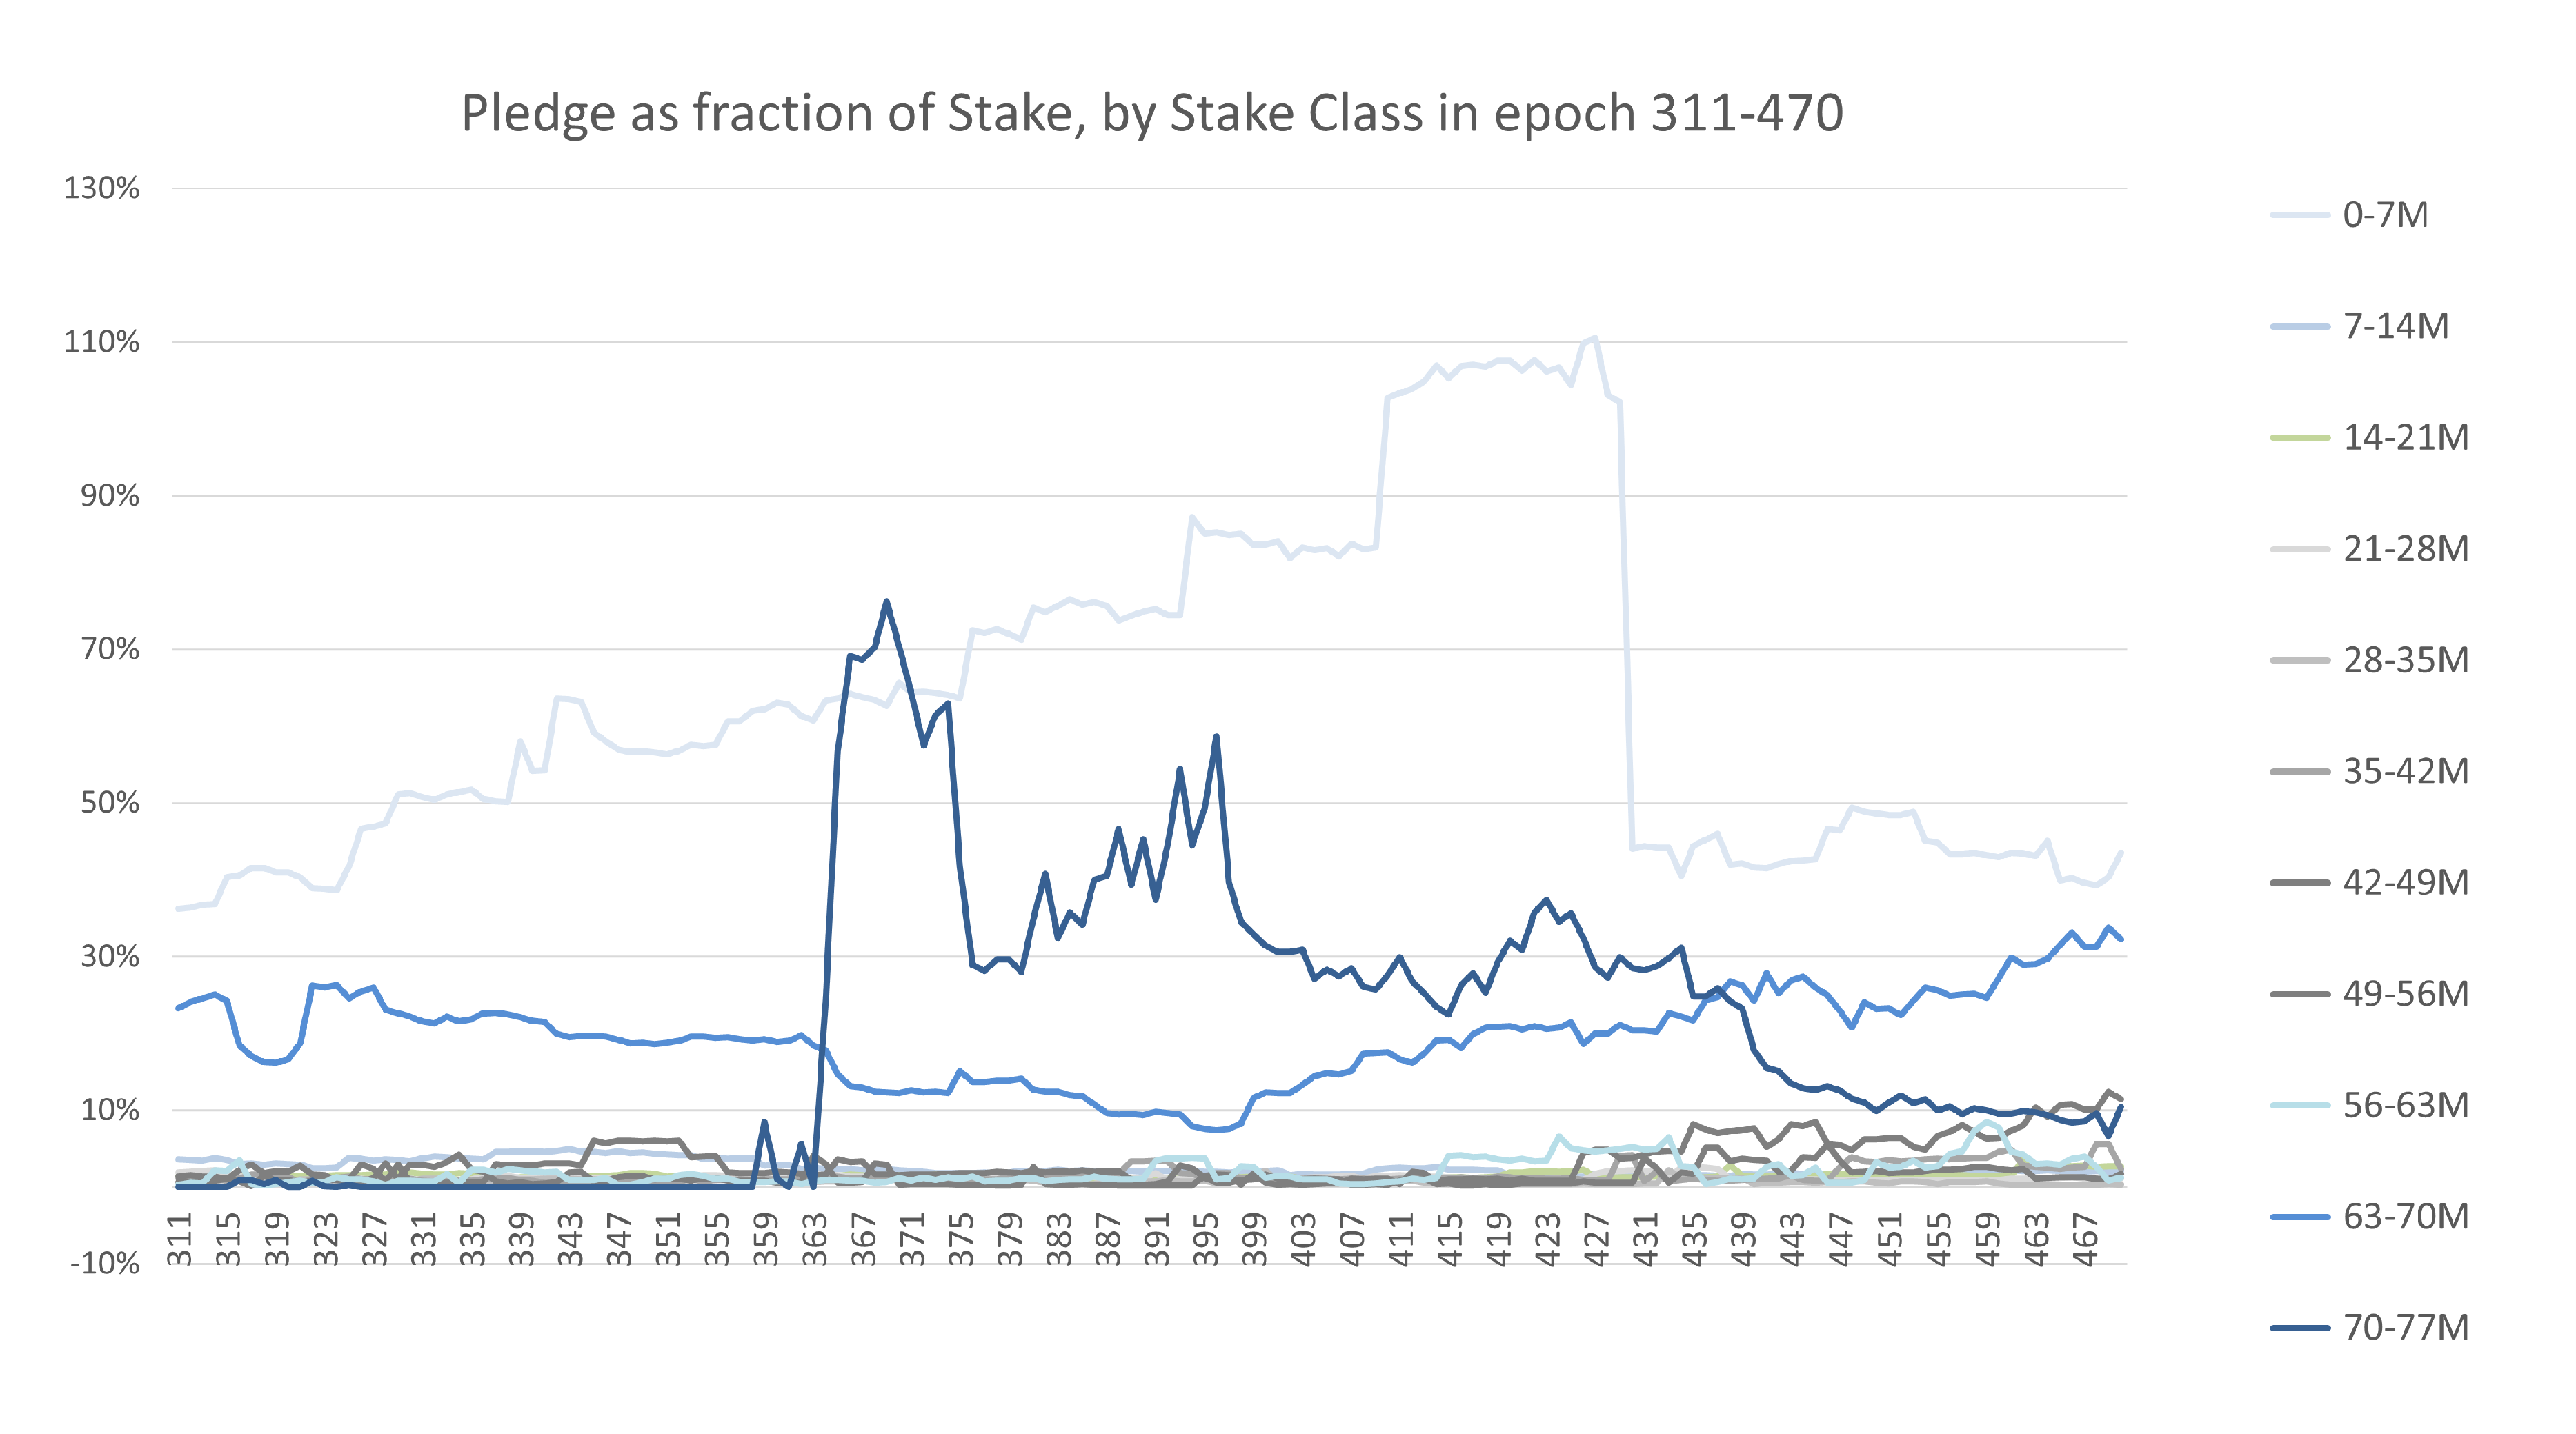
\includegraphics[scale=0.44]{figures/pledgebyrange}\tabularnewline
\end{tabular}\caption{\textbf{Distribution of Stake and Pledge across Stake Classes. }In
the upper chart we see the stake in each class as a percentage of
the stake in all classes. Below, we see the pledge in a class as a
fraction of the Stake in the class.}
\label{fig_pools_by_stake}
\end{figure}

The dynamics of all classes of stake during the period shows a rather
complex and volatile situation, yet there is a clear evidence that
cohorts associated to the largest pools are also those where most
of the stake is concentrated, with an expected gradual shift from
the $\left[63M-70M\right]$ to the $\left[70M-77M\right]$ stake cohort
as the saturation level increased, passing $70M$ due to the growth
of circulating supply. Yet, in the last year or so, no cohort contained
more than 20\% of the active stake. 

In Figure \ref{fig_pools_by_stake}, the lower chart shows how the
pledge has been distributed across the above classes of stake, measured
a percentage of the class stake. We notice larger percentage pledge
for the class containing the smallest pools, and for those containing
the largest ones. This is not surprising. Small pools typically start
with own stake, and the very high percentage of pledge may be apparent,
since they include pools that are not yet or no longer operative,
or not yet or no longer matching their declared pledge. This may explain
why in some moments the pledge appeared even higher than the associated
stake. In any case, pledge in this class has little to no impact on
the amount of rewards received, since for pools with stake lower than
10\% of the saturation a higher pledge proportion yields little to
no advantage. 

Conversely, larger pools are likely to hold more pledge both because
they are more likely to have been created by large holders, or because
their incentive to hold more pledge is the highest among all pools.
Yet recently even the largest classes have an overall percentage of
pledge which is between 30\% and 10\%, while many others have much
less. 

\textbf{Estimates}. To keep the statistics sufficiently synthetic,
we do not use information on how the pledge was distributed within
a class, but just the relative pledge held in the class, over the
stake held in the class. This does not tell us directly how much single
pools own, but can allow us some estimates. If we want an overestimate
of their fees, for example, we can assume that in every class all
pools have the maximum stake. We will also assume they all have the
same percentage pledge. This is likely to be an overestimate as well,
since pledge has for all but the largest, saturated pools, a less
than linear impact on rewards. We can even apply this logic to the
time average of stake and pledge across the whole period, which is
shown in the upper chart of Figure \ref{fig_stakepledgebyclass}.
The histogram corresponds to the following table:

\hspace{-0.85cm}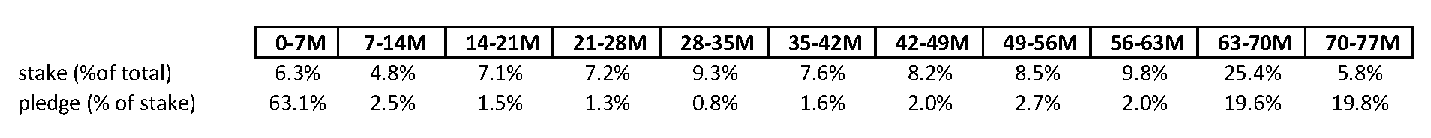
\includegraphics[scale=0.66]{./figures/pools_histogram_table.eps}

This shows that on average, across the period the 0-7M class held
6.3\% of the stake, while pledge in the class was on average 63.1\%
of the stake, while 7-14M pools held 4.8\% of the stake and pledge
was 2.5\% of the stake, and so on. If we apply the above estimate
logic to these data, we treat all the 0-7M pools as if they were 7M
pool with 63.1\% pledge, all 7-14M pools as if they were 14M pools
with 4.8\% stake and so on. Now for each class, we can compute the
amount of rewards as a percentage of the maximum ($\frac{1}{k}$ of
the total rewards). Since we know that the first class weighted for
6.3\% of the stake, the second one for 7.1\% and so on, then we can
compute a weighted average. This is shown in the lower chart of Figure
\ref{fig_stakepledgebyclass}, where it is compared to the $76.9\%%\ensuremath{=\frac{1}{1+a_{0}}}
$ earned by pools with no pledge. Because of the time average, this
rough estimate is not necessarily an overestimate, yet we obtain $78.6\%$,
which is consistent with the $f_{i}$ values in Figure \ref{fandp}
showing that the aggregate incentive adjustment was within $2\%$
of the minimum. 
\begin{figure}[H]
\medskip{}
\begin{tabular}{c}
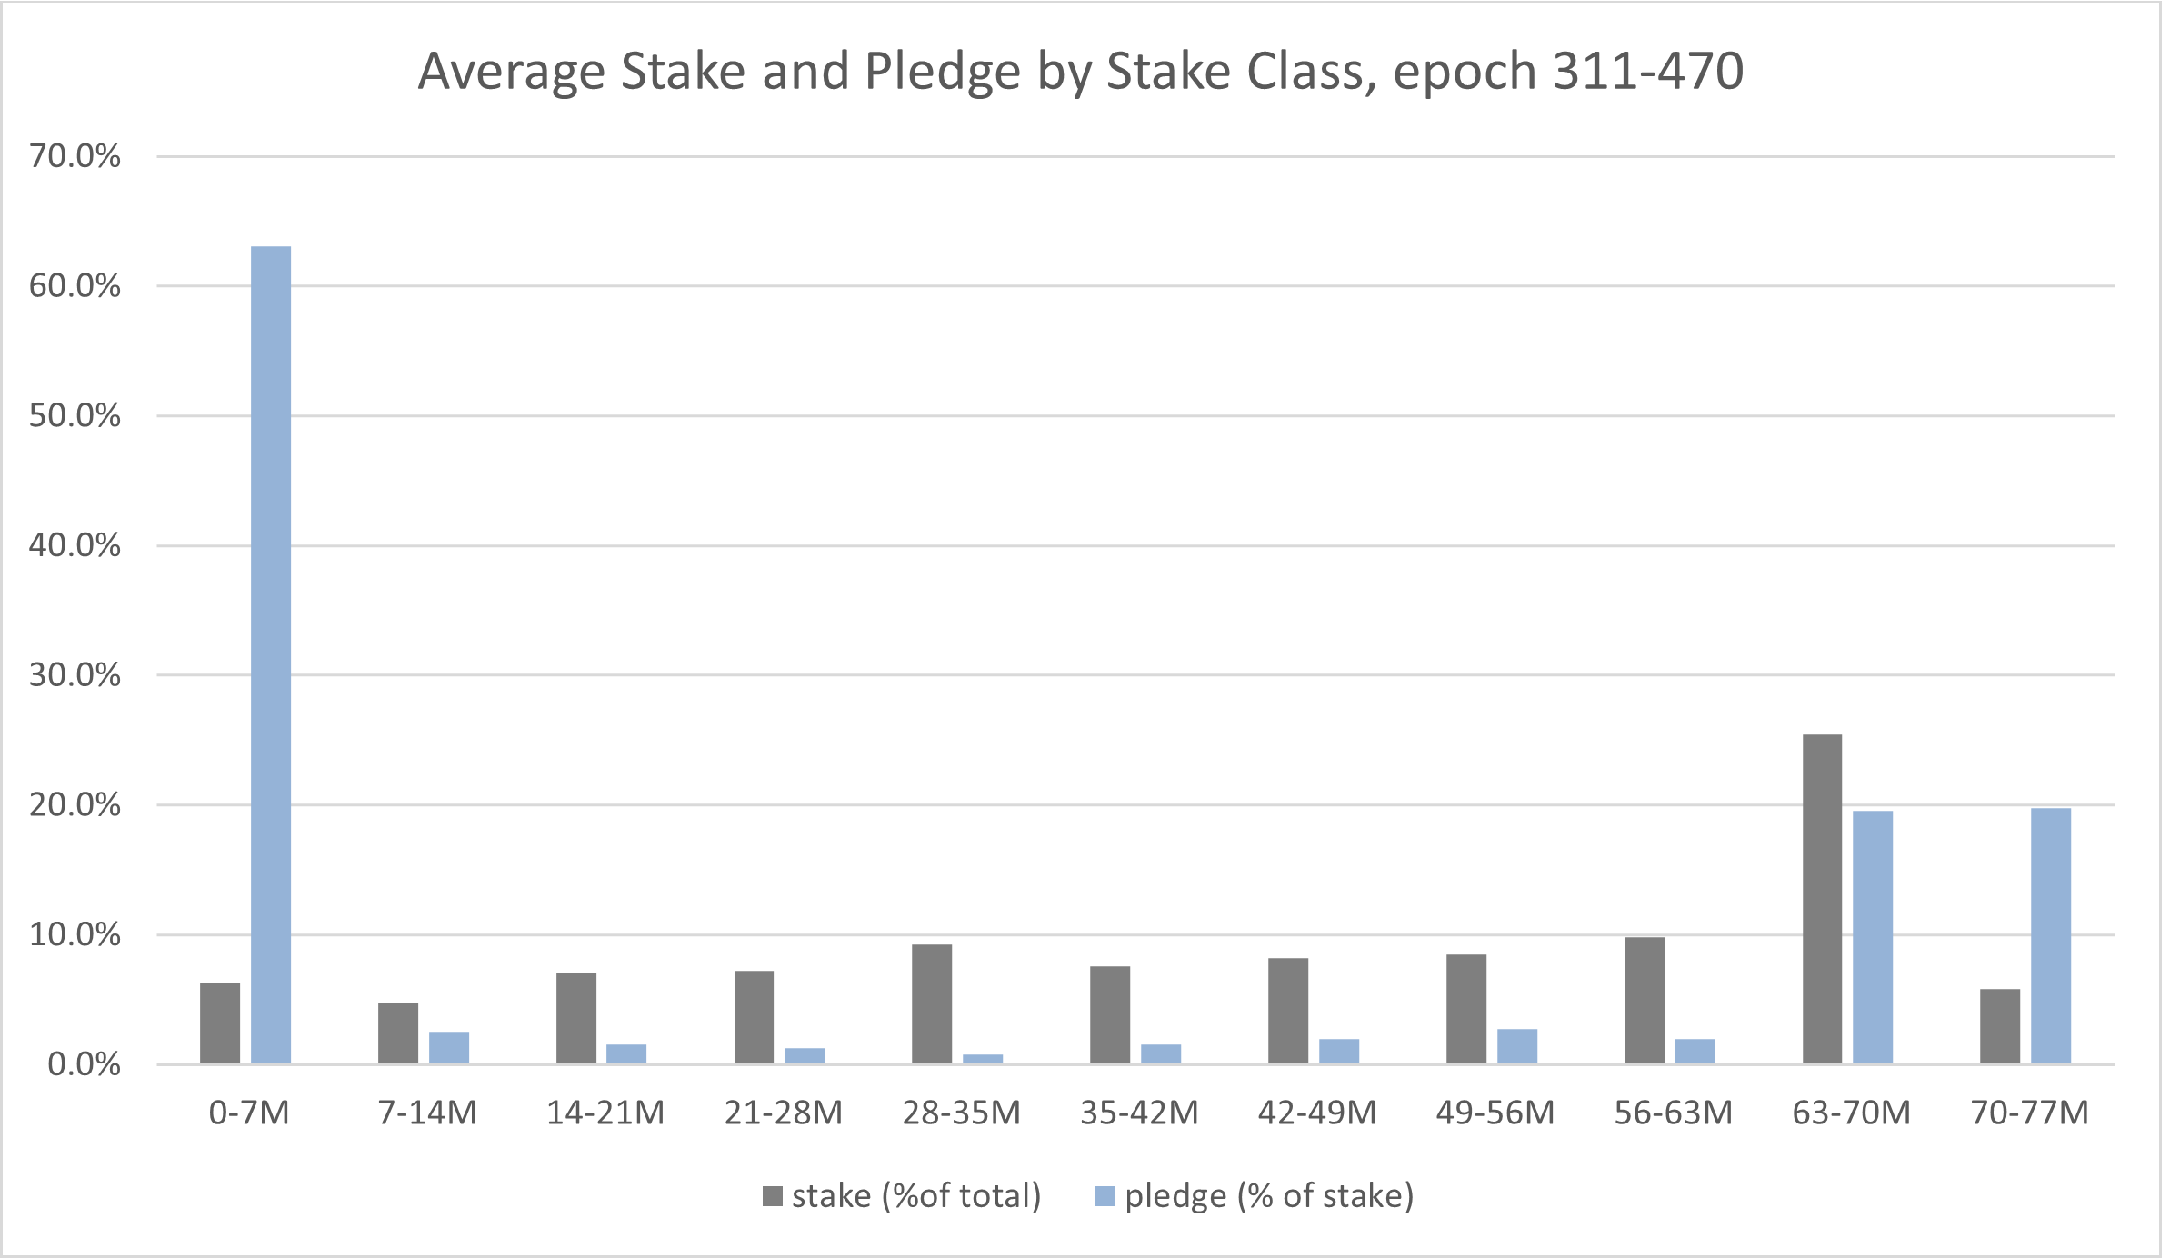
\includegraphics[scale=0.78]{./figures/average_by_class.eps}\tabularnewline
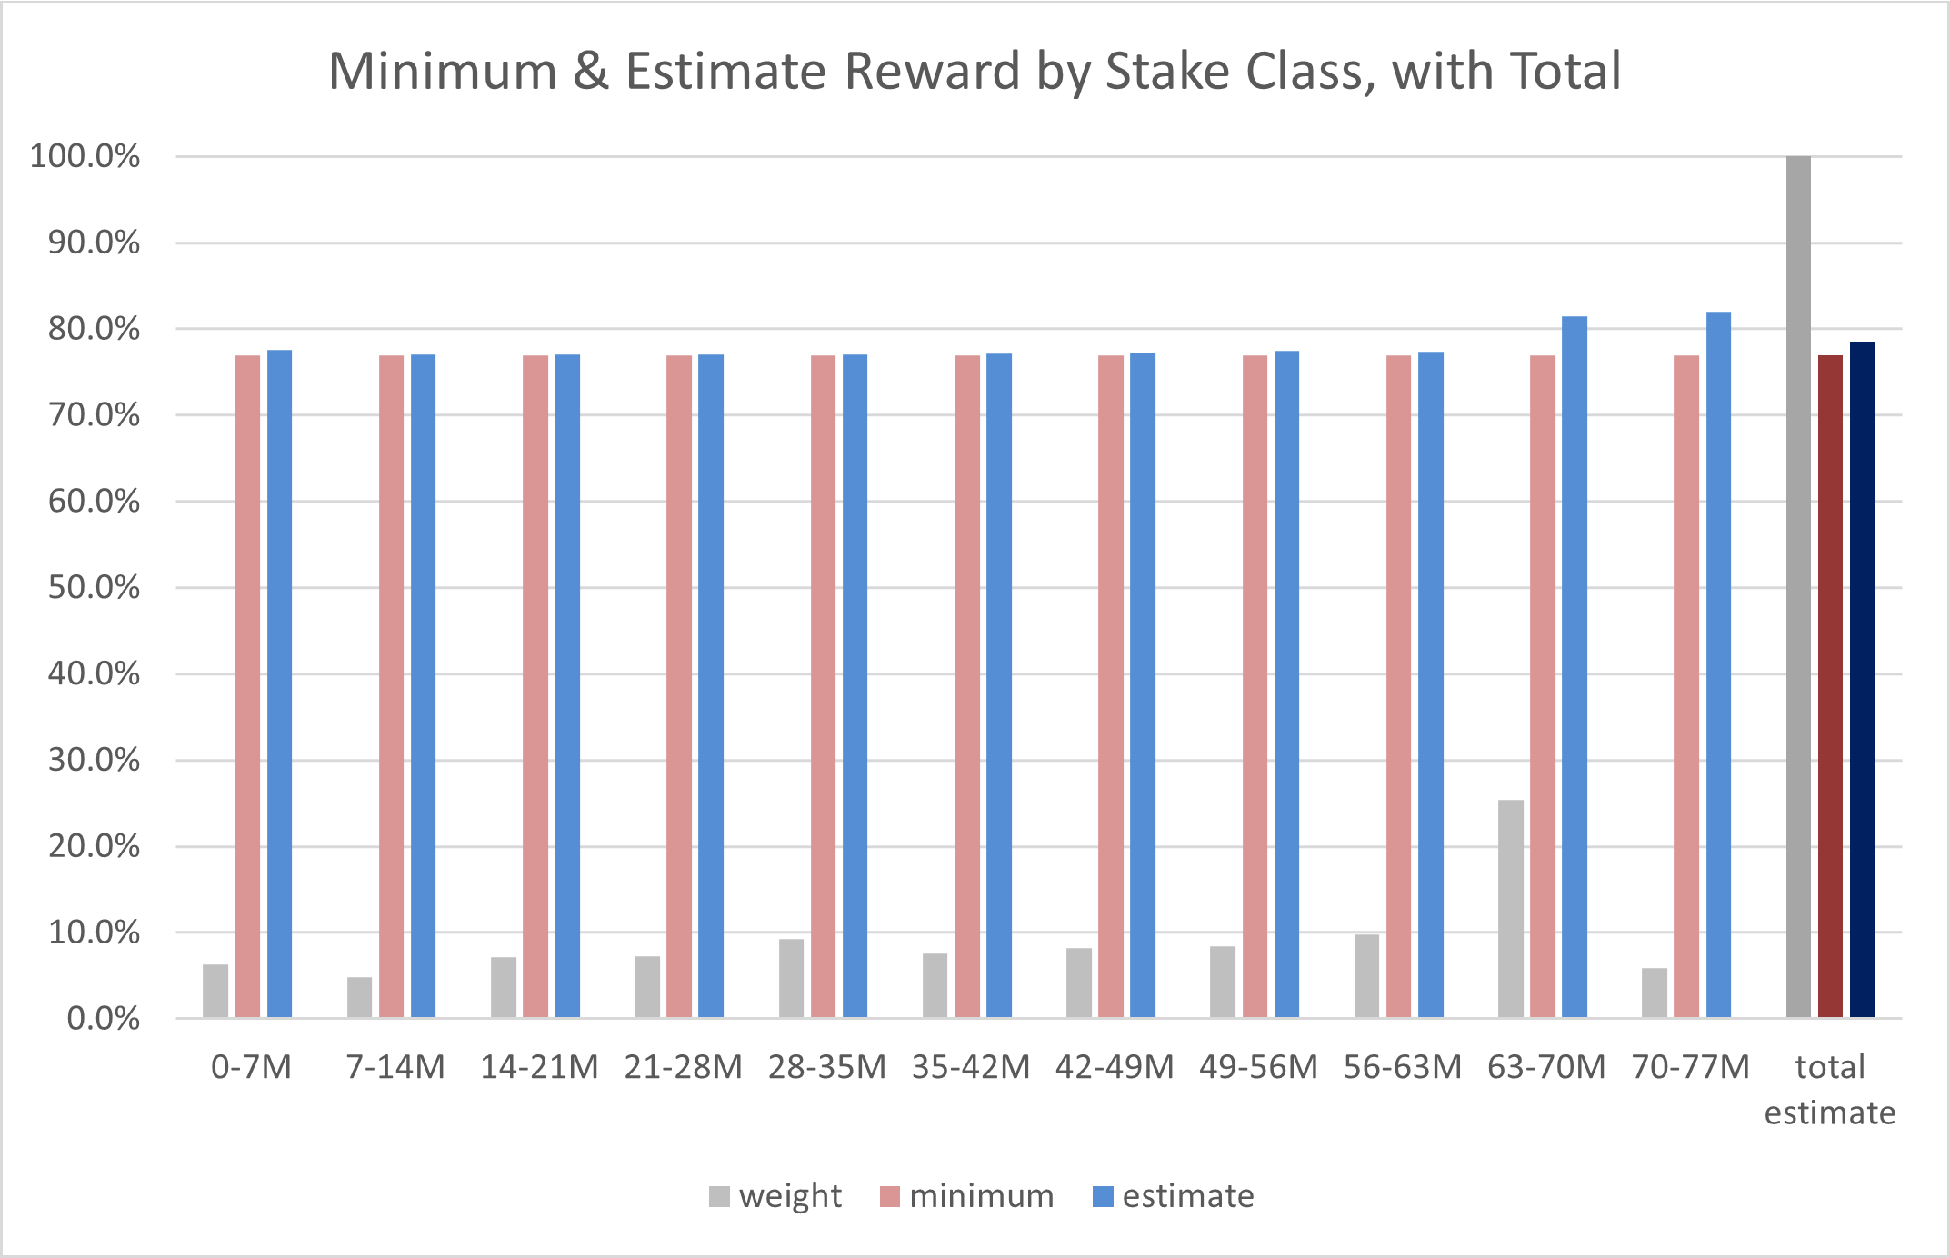
\includegraphics[scale=0.78]{./figures/estimate_by_class.eps}\tabularnewline
\end{tabular}\caption{\textbf{Stake and Pledge Statistics and Reward Estimates. }In the
upper chart we see the time-averages of stake and pledge. Below, we
see estimates of the reward percentages.}
\label{fig_stakepledgebyclass}
\end{figure}

However rough, this statistic support the assumption that the current
level of own stake and its distribution across pools leads to rewards
that, on average, near those of a pool with no own stake. Indeed,
even for large saturated pools, financial optimization may lead to
a low amount of pledge, since for them a higher pledge increases the
total rewards for large pools, but the yield on own capital may be
reduced when increasing the pledge. Thus even large pools may find
it sub-optimal to replace delegated capital with own capital in order
to get the last 23\% of the full reward potential. A precise utility
and cost assessment, and the interplay with parameters setting minimum
costs and margins for individual pools, are left to future research.

\section{Actual Reserves and Treasury Distribution}

The reward incentives have effects on Cardano Tokenomics that go beyond
rewarding differently pools of different stake and pledge. The documentation
in \citet{webdocgeneral} introduces Cardano monetary policy by describing
the Reserves as the difference between the maximal supply of ADA and
the circulating supply, and explaining that ``during each epoch,
a fixed but parameterizable percentage of the remaining reserve is
taken from the reserve and used for epoch rewards and treasury'',
and later on that ``fees from every transaction from all blocks produced
during every epoch go into a virtual 'pot'. A fixed percentage (\textgreek{r})
of the remaining ADA reserves is added to that pot. A certain percentage
(\textgreek{t}) of the pot is sent to the treasury, and the rest is
used as epoch rewards''.

These parameters always had values $\rho=0.003$ and $\tau=0.2$.
The above description leads to a simple mathematical representation
of the Cardano Economic Dynamics. The Pot is funded by Fees $F_{i}$
and the regular release of Reserves $\rho\mathrm{Reserve}$, 
\[
Pot_{i}=F_{i}+\rho\mathrm{Reserve}_{i-1},
\]
 and it is then distributed to Treasury and Rewards in fixed proportions
\begin{align}
\mathrm{Rewards}_{i} & =\left(1-\tau\right)Pot_{i}.\label{eq:distribution}\\
\varDelta\mathrm{Treasury}_{i} & =\tau Pot_{i}\nonumber 
\end{align}
where $\varDelta\mathrm{Treasury}_{i}$ is the increase in the value
of the treasury added at every release. Quantities indexed with $i$
are usually known through epoch $i$. 

The above description leads to a simple fundamental equation for monetary
policy, a formula for the update of Reserves given by 
\begin{align}
\mathrm{Reserve}_{i} & =\mathrm{Reserve}_{i-1}-\rho\mathrm{Reserve}_{i-1}\nonumber \\
 & =\mathrm{Reserve}_{i-1}\left(1-\rho\right),\label{eq:fundamental simple}
\end{align}
In practice there are several additional elements that bring variability.
First of all, $\rho$ is multiplied by a quantity $\eta_{t}$. This
is the aggregate equivalent of the adjustments for pool's performances
seen above. It is given by the ratio between the actual number of
blocks produced in an epoch, and the theoretical value of $21,600$
obtained as the number of slots (seconds) in an epoch multiplied by
the so-called \textit{active slots coefficient} of $5\%$. Also with
the inclusion of $\eta_{i}$, the formula for the update of Reserves
remains simple
\[
\mathrm{Reserve}_{i}=\mathrm{Reserve}_{i-1}\left(1-\rho\eta_{i}\right),
\]
but we are still far from the actual distribution, since we are ignoring
the adjustments to rewards seen in the previous sections. We have
to take into account the effect of the incentive factor $f_{i}$,
and the $p_{i}$ rescaling. So the actual amount of Rewards distributed
is reduced by the adjustments, and formula \eqref{eq:distribution}
becomes

\begin{align*}
\mathrm{Rewards}_{i} & =f_{i}p_{i}\left(1-\tau\right)Pot_{i}\\
\varDelta\mathrm{Treasury}_{i} & =\tau Pot_{i}
\end{align*}
Thus, the proportion between the Treasury increase and the Rewards
is not the one between $\tau$ and $1-\tau$. The fraction of the
theoretical release devoted to the Treasury has really been around
$\tau=20\%$, but reducing Rewards to a fraction $f_{i}p_{i}\left(1-\tau\right)$
rather than just $\left(1-\tau\right)$ changes the actual proportions.
\begin{figure}[H]
\bigskip{}

\hspace{-0.2cm}%
\begin{tabular}{cc}
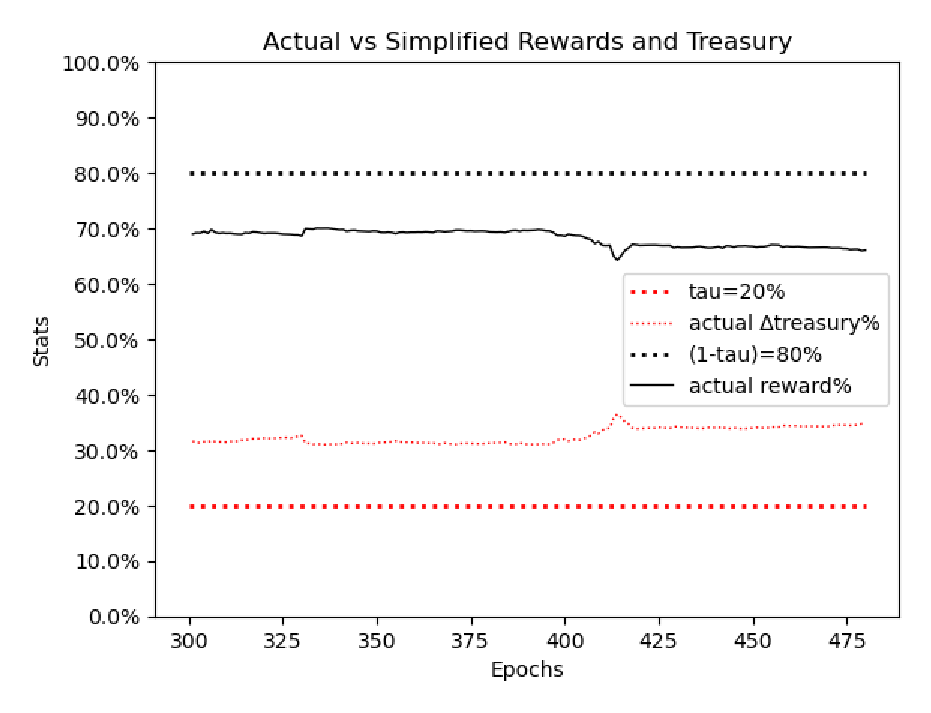
\includegraphics[scale=0.46]{./figures/actualvssimplified_rewards_and_treasury.eps} & 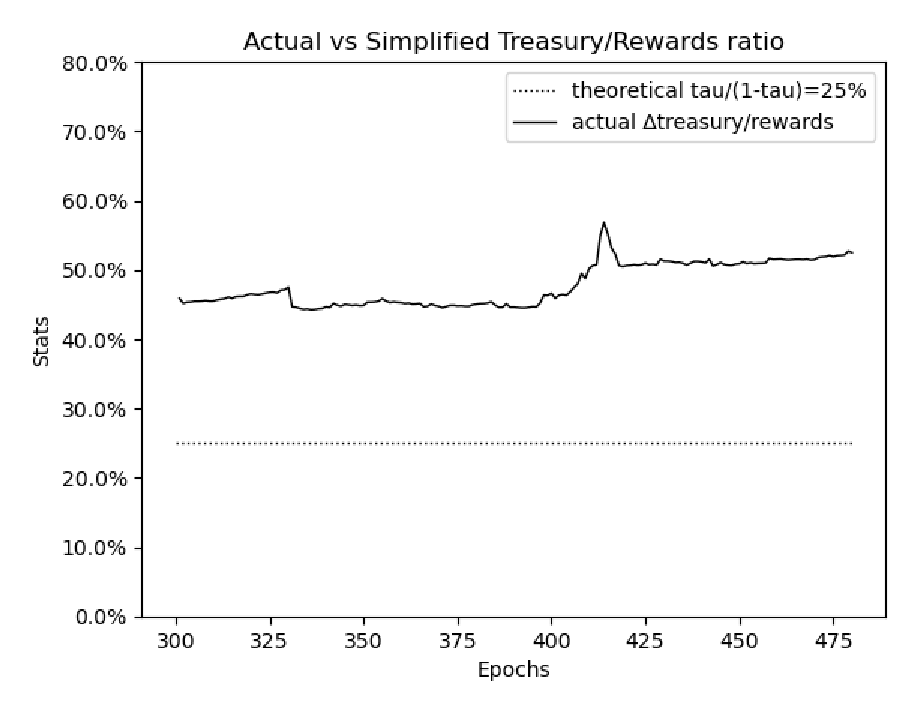
\includegraphics[scale=0.46]{./figures/actualvssimplified_trerew_ratio.eps}\tabularnewline
\end{tabular}\caption{\textbf{Actual vs Theoretical Rewards and Treasury}}
\label{rewards_and_treasury}
\end{figure}

Look at Figure \ref{rewards_and_treasury}. On the left we see that,
rather than $80\%$ of the release, Rewards have been between a bit
less than 65\% and little more than 70\%, with Treasury taking a fraction
approximately between $30\%$ and $35\%$. Thus, as we see on the
right, the proportion between the growth of Treasury and the Rewards,
that in principle should be $\frac{\tau}{1-\tau}=25\%$, has often
been more than 50\%. 

A more precise description of the effect of rewards adjustments is
given in Figure \ref{rewards_and_treasury_1}, that breaks down the
effect for $f_{i}$ and $p_{i}$. We can see that without incentives,
equivalent to setting $f_{i}=1$, but with the $p_{i}$ rescaling,
rewards would be be nearer to the theoretical value of $80\%$, and
even more if instead we had incentives $f_{i}$ but no $p_{i}$ rescaling.
This is consistent with the results of the previous sections. If there
were neither $f_{i}$ nor $p_{i}$ adjustments, the distribution would
be very close to the theoretical values, in spite of some elements
of variability, such as Fees or the treatment of unpaid rewards and
unreturned deposits, that are rather small and not represented explicitly
here. 

\begin{figure}[H]
\smallskip{}

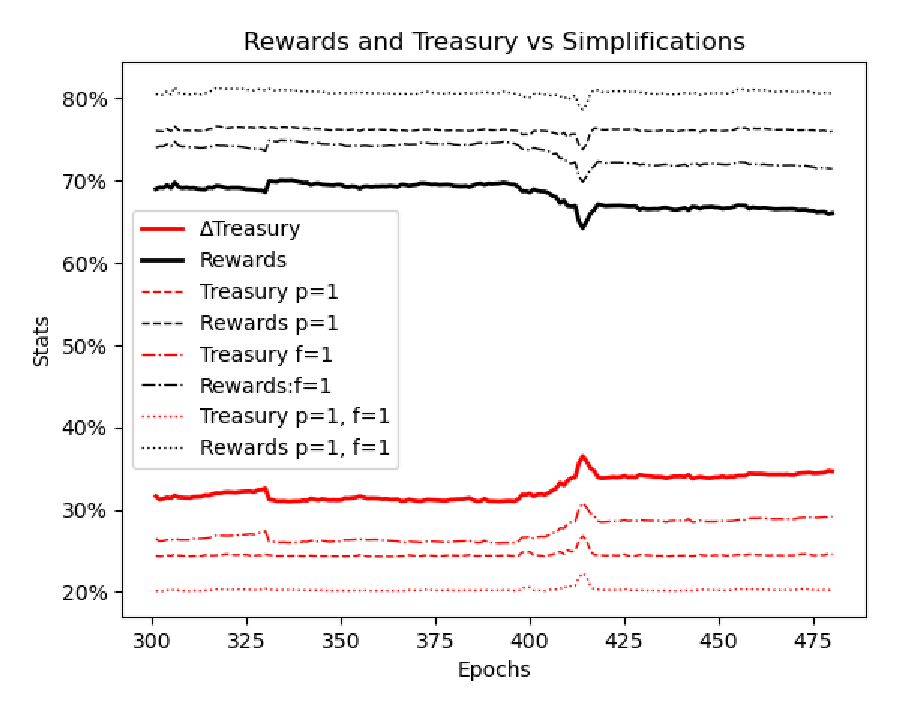
\includegraphics[scale=0.88]{./figures/actualvssimplified_rewards_and_treasury_breakdown.eps}
\caption{\textbf{Rewards and Treasury. Breakdown of Adjustments.} }
\label{rewards_and_treasury_1}
\end{figure}

What happens to the amounts which are not paid out as Rewards? They
stay with the Reserves, making the actual release lower than the one
dictated by the monetary expansion parameter $\rho$. This is another
difference between simplified descriptions of the tokenomics and the
reality. In Figure \ref{actual_and_simplified_reserves}, left chart,
we see the actual dynamics Reserves had in the last few years, compared
to the predictions of simplified representations, where the $f_{i},p_{i}$,
and potentially also the $\eta_{i}$ adjustment are ignored. The difference
is material, and the most relevant contribution to this difference
does not come from ignoring $\eta_{i}$, but from ignoring the effect
of reward adjustment. This effect alone leads to a difference of almost
1.5B ADA in the amount of reserves over 2.5 years. Ignoring $\eta_{i}$
as well leads only to an additional difference of little more than
100M ADA. 

\begin{figure}[H]
\hspace{-0.2cm}%
\begin{tabular}{cc|}
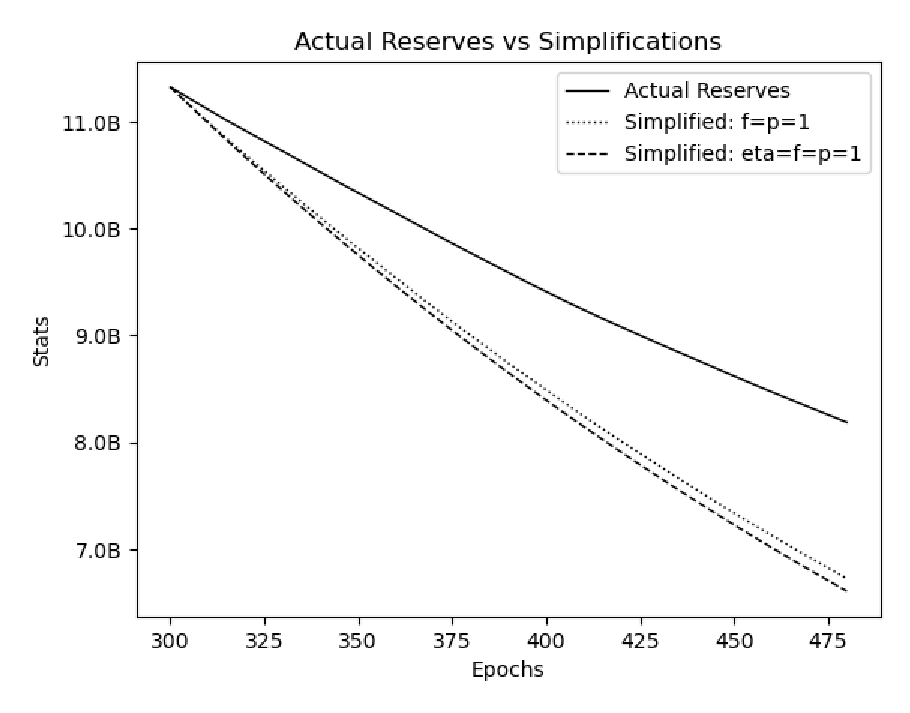
\includegraphics[scale=0.47]{./figures/actual_and_simplified_reserves.eps} & 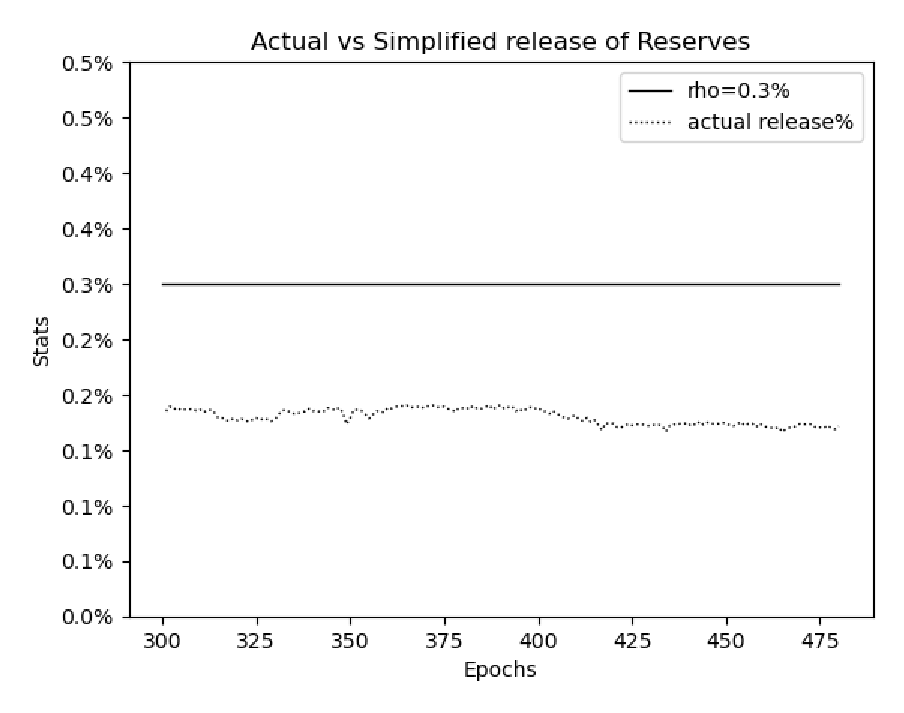
\includegraphics[scale=0.47]{./figures/actualvssimplified_eta.eps}\tabularnewline
\end{tabular}
\caption{\textbf{Actual Reserves vs Simplifications}}
\label{actual_and_simplified_reserves}\medskip{}
\end{figure}

This clarifies that the release from Reserves does not happen at a
fixed rate equal to $\rho=0.3\%$ but at a variable rate, lower than
$\rho$ and ranging, in the period analyzed, between $0.165\%$ and
$0.185\%$. This means that in some cases the reward adjustments can
make the release be only little more than half of the theoretical
value, as we can see in the right chart of Figure \ref{actual_and_simplified_reserves}. 

Taking into account also the impact of $f_{i}$ and $p_{i}$, the
formula for the update of Reserves become much more complicated, since
we have to take into account the undistributed part of $Pot_{i}$
returning to Reserves, including a component from fees $F_{i}$:
\begin{align*}
\mathrm{Reserve}_{i} & =\mathrm{Reserve}_{i-1}\left(1-\rho\eta_{i}\right)+\left(1-\tau\right)\left(F_{i}+\rho\eta_{i}\mathrm{Reserve}_{i-1}\right)\left(1-p_{i}f_{i}\right)\\
 & =\mathrm{Reserve}_{i-1}\left(1-\rho\eta_{i}\left(\tau-\left(1-\tau\right)p_{i}f_{i}\right)\right)+\left(1-\tau\right)F_{i}\left(1-p_{i}f_{i}\right)
\end{align*}

\begin{figure}[ht]

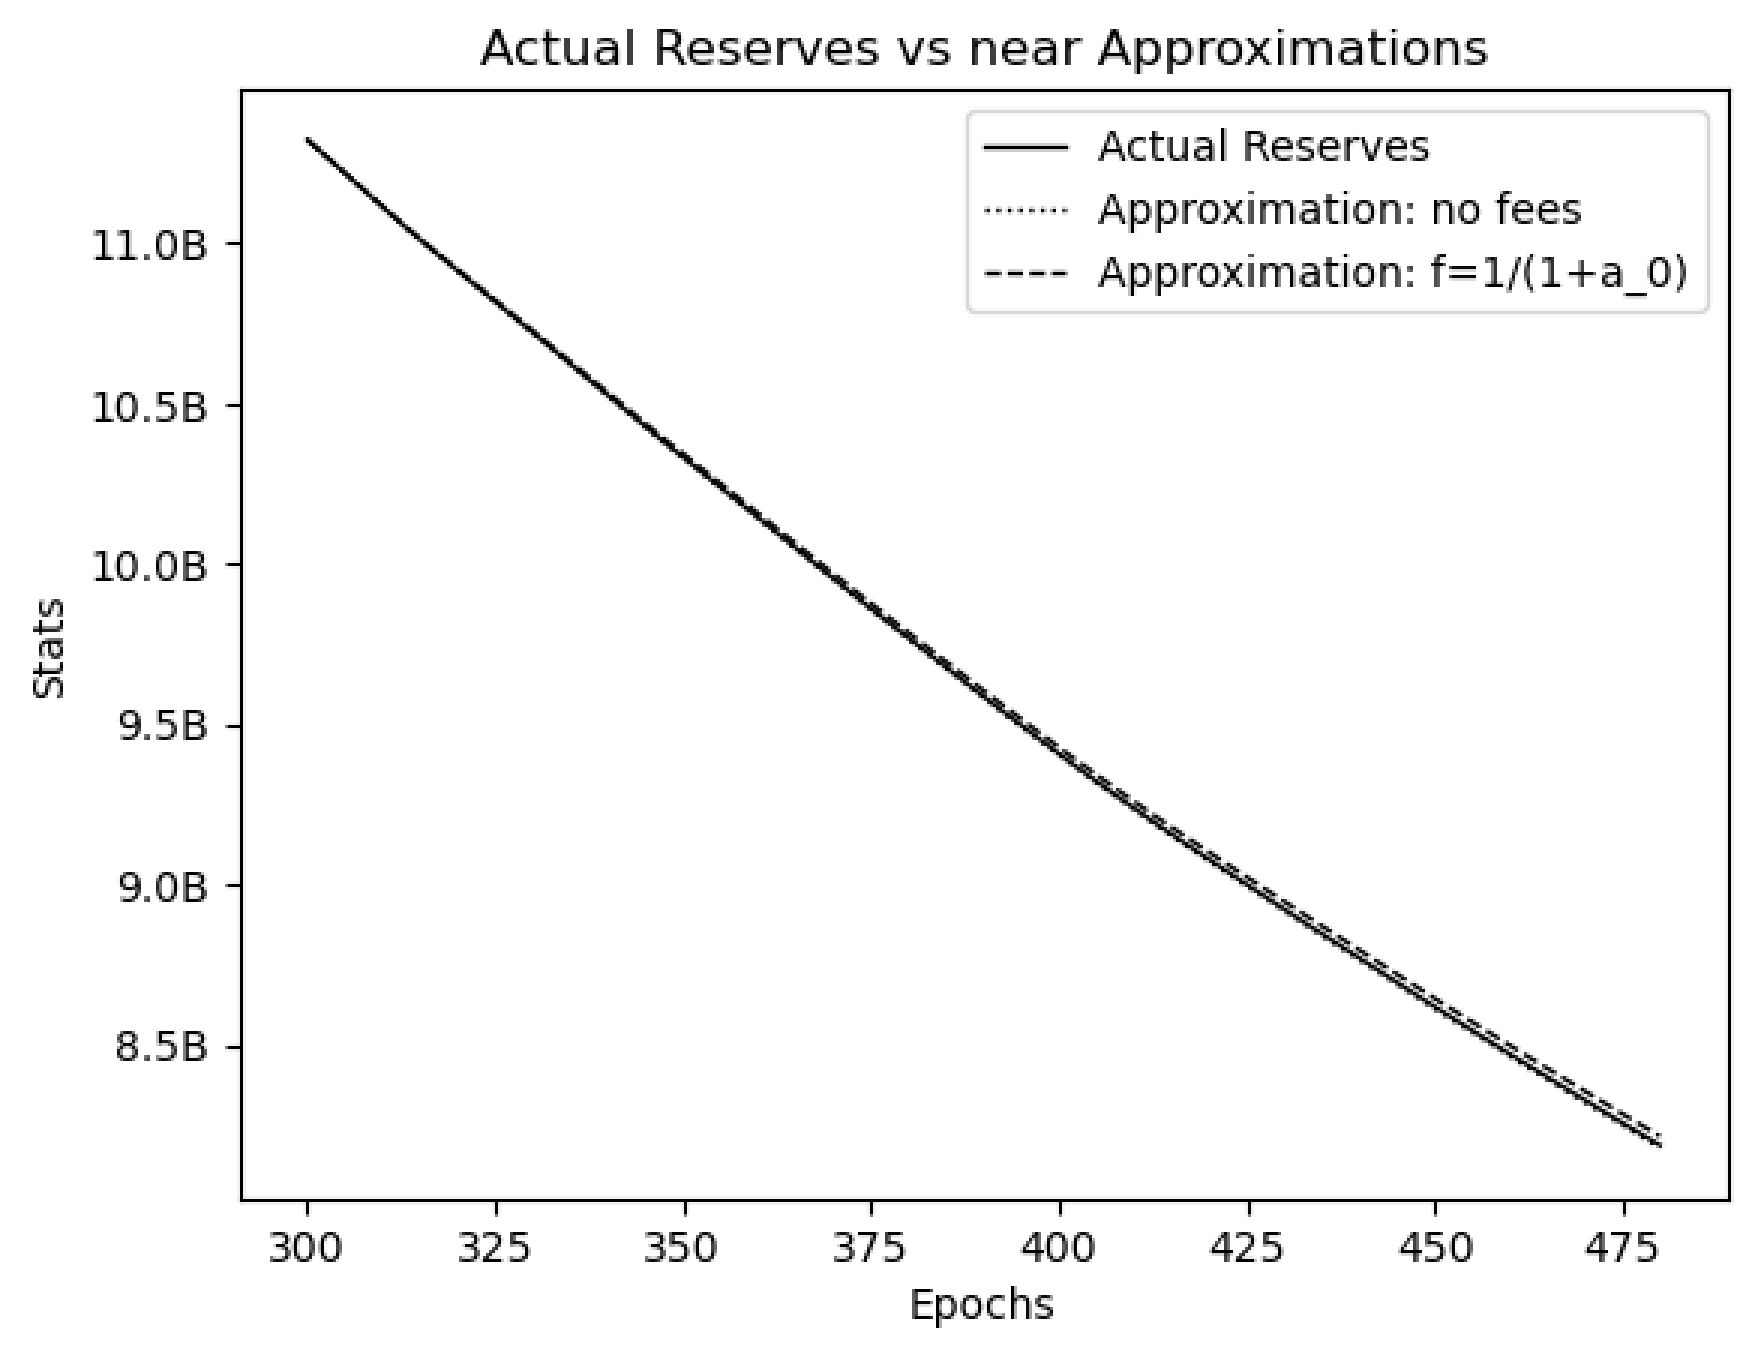
\includegraphics[scale=0.8]{"./figures/actual_and_approximated_reserves.eps"}
\caption{\textbf{Actual Reserves vs Near Approximations}}
\label{actual and approximated reserves}\smallskip{}
\end{figure}
It is useful to see the relevance of the different parts of this equation.
So far we have seen that some simplifications, like ignoring the effect
of the incentive parameterization on the monetary policy, leads to
massive errors. However, there are also approximations that simplify
the picture with a very limited practical impact. Here the most relevant
is to exclude the $F_{i}$ component from the reserve update, leading
to a simpler equation
\begin{align*}
\mathrm{Reserve}_{i} & =\mathrm{Reserve}_{i-1}-\rho\eta_{i}\mathrm{Reserve}_{i-1}+\rho\eta_{i}\mathrm{Reserve}_{i-1}\left(1-\tau\right)\left(1-p_{i}f_{i}\right)\\
 & =\mathrm{Reserve}_{i-1}\left(1-\rho\eta_{i}\left(\tau-\left(1-\tau\right)p_{i}f_{i}\right)\right).
\end{align*}
This equation has a trivial solution
\[
\mathrm{Reserve}_{i}=\mathrm{Reserve}_{0}\prod_{j=1}^{i}\left(1-\rho\eta_{i}\left(\tau-\left(1-\tau\right)p_{i}f_{i}\right)\right),
\]
expressing directly current reserves in terms of their level at an
initial epoch. This is equation allows also to project easily Reserves
into the future. However, we have to remember not only that we still
have to consider the impact of Fees, currently very small but potentially
relevant in the future, but also that the elements introduced, compared
to the simplified version in (\vref{eq:fundamental simple}), are
stochastic, which meas that they vary randomly.

We have analyzed their statistical properties and leveraged this analysis
to model them as stochastic processes. We considered both a discrete-time
setting, where epochs correspond to finite-difference time steps,
and a continuous-time framework, obtained by taking the epoch frequency
to the limit. This has a contained impact, that we assessed both analytically
and in simulation, while making the system much more tractable. As
anticipated above, $\eta_{i}$ and $f_{i}$ exhibit smooth dynamics
that are well-represented by continuous stochastic processes. While
$p_{i}$ could instead be modeled as a jump-diffusion process, incorporating
a jump component governed by a compound Poisson process, when considered
jointly with the other processes, the resulting dynamics remains smooth.

Our analysis was conducted to gain a deeper understanding of Cardano
economic parameters, particularly to clarify their interactions in
the context of the current decentralization of governance. At the
same time, it serves as both a foundation and a blueprint for the
stochastic modeling of the system---an equally crucial requirement
for the future governance of decentralized ecosystems. This topic
will be explored further in the follow-up to this document.

\section*{Conclusions and Perspectives}

In this paper we analyzed staking incentives, showing how the parameters
for pledge influence and desired stake size have very differentiated
effects on the rewards of pools with different features. We looked
at the impact of stake calculations, and of the actual pool distribution,
on rewards. Finally we analyzed how the dynamics of reserves, rewards
and treasury is affected by incentives and stake calculations. We
used simple math, economics, and data analysis, striving to keep complexity
to a minimum. We have made the paper available to the community to
foster discussion and improvements at https://github.com/cardano-foundation/cardano-economic-parameter-insights.

This paper is part of a larger research that extends some of the above
analysis, including a more detailed investigation of the resource
optimization problem faced by pools, taking into account also the
parameters limiting pools choices, such as minimum costs and margins,
and the long term impact of rewards. The analysis of the actual dynamics
of variables such as reserves and rewards extends to measuring their
statistical properties and modeling them using stochastic finite-difference
or differential equations. This is facilitated by Cardano\textquoteright s
rigorous parameterization, as highlighted also in \citet{hoskinson2018ama}.
This topic is relevant for projecting and simulating the effect of
governance choices on the long-term evolution of the system, properly
accounting for probabilistic uncertainty. 

\bibliographystyle{elsarticle-num-names}
\bibliography{cardano_bibliography}

\end{document}
